\documentclass[a4paper]{tufte-book}\usepackage[]{graphicx}\usepackage[]{xcolor}
% maxwidth is the original width if it is less than linewidth
% otherwise use linewidth (to make sure the graphics do not exceed the margin)
\makeatletter
\def\maxwidth{ %
  \ifdim\Gin@nat@width>\linewidth
    \linewidth
  \else
    \Gin@nat@width
  \fi
}
\makeatother

\definecolor{fgcolor}{rgb}{0.345, 0.345, 0.345}
\newcommand{\hlnum}[1]{\textcolor[rgb]{0.686,0.059,0.569}{#1}}%
\newcommand{\hlsng}[1]{\textcolor[rgb]{0.192,0.494,0.8}{#1}}%
\newcommand{\hlcom}[1]{\textcolor[rgb]{0.678,0.584,0.686}{\textit{#1}}}%
\newcommand{\hlopt}[1]{\textcolor[rgb]{0,0,0}{#1}}%
\newcommand{\hldef}[1]{\textcolor[rgb]{0.345,0.345,0.345}{#1}}%
\newcommand{\hlkwa}[1]{\textcolor[rgb]{0.161,0.373,0.58}{\textbf{#1}}}%
\newcommand{\hlkwb}[1]{\textcolor[rgb]{0.69,0.353,0.396}{#1}}%
\newcommand{\hlkwc}[1]{\textcolor[rgb]{0.333,0.667,0.333}{#1}}%
\newcommand{\hlkwd}[1]{\textcolor[rgb]{0.737,0.353,0.396}{\textbf{#1}}}%
\let\hlipl\hlkwb

\usepackage{framed}
\makeatletter
\newenvironment{kframe}{%
 \def\at@end@of@kframe{}%
 \ifinner\ifhmode%
  \def\at@end@of@kframe{\end{minipage}}%
  \begin{minipage}{\columnwidth}%
 \fi\fi%
 \def\FrameCommand##1{\hskip\@totalleftmargin \hskip-\fboxsep
 \colorbox{shadecolor}{##1}\hskip-\fboxsep
     % There is no \\@totalrightmargin, so:
     \hskip-\linewidth \hskip-\@totalleftmargin \hskip\columnwidth}%
 \MakeFramed {\advance\hsize-\width
   \@totalleftmargin\z@ \linewidth\hsize
   \@setminipage}}%
 {\par\unskip\endMakeFramed%
 \at@end@of@kframe}
\makeatother

\definecolor{shadecolor}{rgb}{.97, .97, .97}
\definecolor{messagecolor}{rgb}{0, 0, 0}
\definecolor{warningcolor}{rgb}{1, 0, 1}
\definecolor{errorcolor}{rgb}{1, 0, 0}
\newenvironment{knitrout}{}{} % an empty environment to be redefined in TeX

\usepackage{alltt}
\hypersetup{colorlinks}% uncomment this line if you prefer colored hyperlinks (e.g., for onscreen viewing)

\usepackage{setspace}
\usepackage{parskip}


\makeatletter
% Paragraph indentation and separation for normal text
\renewcommand{\@tufte@reset@par}{%
  \setlength{\RaggedRightParindent}{1.0pc}%
  \setlength{\JustifyingParindent}{1.0pc}%
  \setlength{\parindent}{1em}%
  \setlength{\parskip}{0.3\baselineskip}%
}
\@tufte@reset@par
% 
% % Paragraph indentation and separation for marginal text
% \renewcommand{\@tufte@margin@par}{%
%   \setlength{\RaggedRightParindent}{0.5pc}%
%   \setlength{\JustifyingParindent}{0.5pc}%
%   \setlength{\parindent}{0pt}%
%   \setlength{\parskip}{\baselineskip}%
% }
% \makeatother

% Define a new counter for theorems, lemmas, remarks, etc.
\newcounter{mycounter}[chapter] % Reset counter at the start of each chapter
\renewcommand{\themycounter}{\thechapter.\arabic{mycounter}}
\NewDocumentCommand{\mypar}{som}{%
  \refstepcounter{mycounter}%
  \par\medskip\noindent\textbf{#3 \themycounter}%
    \IfBooleanF{#1}{\IfValueT{#2}{\space(#2)}}\textbf{.}%
}

% Terms
\newcommand{\term}[1]{\textbf{#1}}

% Hyperlinks
\usepackage{hyperref}
\usepackage[nospace]{varioref}

% After proofs
\newcommand*{\QED}[1][$\diamondsuit$]{%
\leavevmode\unskip\penalty9999 \hbox{}\nobreak\hfill
    \quad\hbox{#1}%
}

% After comments / exercises
\newcommand*{\parend}[1][$\diamondsuit$]{%
\leavevmode\unskip\penalty9999 \hbox{}\nobreak\hfill
    \quad\hbox{#1}%
}

\renewcommand{\bibname}{References}

\title[Quantitative methodology]{{%
  \setlength{\parindent}{0pt}%
  Quantitative\\
  methodology\\%
  \vspace{1.8cm}%
  {\Huge An introduction}\\%
  \vspace{1.8cm}
  {\huge Autumn 2025}
}}
\date{2020--2025}
\author{Jan Vanhove}
\publisher{University of Fribourg}

\usepackage[export]{adjustbox}

\usepackage{amsmath}
\usepackage{amsfonts}
\usepackage{amssymb}
\usepackage{amsthm}
\usepackage{booktabs}
% \usepackage{mathastext}
\usepackage{mathpazo}
\usepackage{varioref}
\usepackage{bm}
% \renewcommand*{\reftextfaceafter}{on the next page} % Prevents "on the facing page"
% \renewcommand*{\reftextfacebefore}{on the previous page}

% Algorithms
\usepackage[linesnumbered,boxed,vlined,algochapter]{algorithm2e}
\SetArgSty{textup}
\setlength{\algomargin}{1.5em}
\SetAlCapSkip{1em}

\setcounter{secnumdepth}{3}
\setcounter{tocdepth}{1}

\makeatletter
\@addtoreset{chapter}{part}
\IfFileExists{upquote.sty}{\usepackage{upquote}}{}
\begin{document}

\frontmatter

\maketitle

\newpage
\begin{fullwidth}
~\vfill
\thispagestyle{empty}
\setlength{\parindent}{0pt}
\setlength{\parskip}{\baselineskip}
\textit{Quantitative methodology: An introduction} \copyright\ 2020--2025 by Jan Vanhove is licensed under Creative Commons Attribution-NonCommercial 4.0 International. \\
To view a copy of this license, visit \url{https://creativecommons.org/licenses/by-nc/4.0/}. \\
\url{jan.vanhove@unifr.ch} \\
\url{https://janhove.github.io}


% \par\smallcaps{Published by \thanklesspublisher}

% \par\smallcaps{tufte-latex.googlecode.com}

% \par Licensed under the Apache License, Version 2.0 (the ``License''); you may not
% use this file except in compliance with the License. You may obtain a copy
% of the License at \url{http://www.apache.org/licenses/LICENSE-2.0}. Unless
% required by applicable law or agreed to in writing, software distributed
% under the License is distributed on an \smallcaps{``AS IS'' BASIS, WITHOUT
% WARRANTIES OR CONDITIONS OF ANY KIND}, either express or implied. See the
% License for the specific language governing permissions and limitations
% under the License.\index{license}

% \par\textit{First printing, \monthyear}
\end{fullwidth}


\chapter{Preface}
The principal goal of this class is to impart the fundamentals of
quantitative research. Our focus will be on \textbf{drawing causal conclusions}
from data---when are causal conclusions licensed, what are typical pitfalls
when drawing causal conclusions,
and how can you design and optimise studies that avoid these pitfalls?
Throughout, it is imperative that you not only understand the recommendations
given in this booklet but also the \textbf{logic} behind them.
There are two reasons for this.

First, you need to know when the recommendations apply and when they don't.
You might get away with just memorising the recommendations and their scope
for now. But in a couple of months, you're bound to apply them where they don't make
any sense.
Understand the logic behind the recommendations, and you'll be better 
able to weigh your options.

Second, many researchers in the social sciences---even seasoned ones---operate
on rules of thumb, so \emph{they} inevitably end up applying recommendations they've 
picked up somewhere in situations where they don't apply. You need to be able
to make an informed judgement about the research carried out by others and
cogently argue for this judgement. A simple \textit{I took this class that taught
me that you shouldn't control for colliders} won't do.
(You'll learn about colliders and why you shouldn't control for them soon enough.)

In this class, we'll cover the contents of this lecture script.
In addition, we'll spend two sessions on questionnaire design.
Furthermore, in the homework assignments, you'll learn how to visualise data 
using state-of-the-art software. 
These graphing assignments are available from \url{https://janhove.github.io/graphs}.

I occasionally refer to some blog entries I wrote.
These links are clickable in the PDF version of this booklet,
but in case you're reading this from paper, all blog entries
can be found at \url{https://janhove.github.io}.

\medskip

\begin{flushright}
Jan Vanhove\\
\href{mailto:jan.vanhove@unifr.ch}{\texttt{jan.vanhove@unifr.ch}}\\
\url{https://janhove.github.io}
\end{flushright}

{\fontsize{9.5pt}{11pt}\selectfont
  \tableofcontents
}





\mainmatter


\chapter{Association and causality}\label{ch:causality}

\section{Two examples}
Below are two examples of empirical findings 
along with conclusions that someone could draw from them.
Answer the following questions for both of these examples.

\begin{enumerate}
  \item Does the conclusion follow logically from the finding?
        If not, what are some plausible alternative explanations for the finding?
  \item Which additional finding would strengthen the conclusions?
  \item Which additional finding would call the conclusion into question?
\end{enumerate}

\mypar[Receptive multilingualism in Scandinavia]{Example}
When talking their respective native languages, Danes understand
Swedes better than the other way around. Furthermore, Danes
like Swedish better than Swedes do Danish \citep[e.g.,][]{Delsing2005}.

Conclusion: 
Danes understand Swedes better than the other way around 
because they like the language better.\marginnote{The diamond symbol signals where an example, exercise, remark, definition and such like ends.}
\parend

\mypar[Content and language integrated learning]{Example}
Pupils in \textit{Content and Language Integrated Learning} (\textsc{clil}) programmes 
in Andalusia perform better on English proficiency tests 
than other Andalusian pupils \citep{Lorenzo2010}.

Conclusion: 
Taking \textsc{clil} classes improves pupils' English proficiency.
\parend

\newpage

In both examples, an \term{association} of some sort is found in the data,
and a \term{causal explanation} for this association is put forward: 
Not only do Danes both understand and like Swedish better than Swedes do Danish (association), 
it's suggested that one reason why they understand the other language better is that they like it better (explanation).
Similarly, not only do \textsc{clil} pupils in Andalusia outperform non-\textsc{clil} pupils (association),
it's suggested that they outperform them \emph{because} of the \textsc{clil} programme (explanation).

Uncovering associations and drawing causal conclusions from them is a key
goal in empirical research. But it's also fraught with difficulty: after a
moment's thought, you'll often be able to come up with alternative explanations
for the findings. To the extent that there exist more, and more plausible,
alternative explanations, the causal explanation proferred becomes more tenuous:
The causal claim may still be correct, but in the presence of competing explanations,
it can't be \emph{shown} to be correct---that is, there isn't much \term{evidence}
for the claim.
A key goal when designing an empirical study is to reduce the number and the
plausibility of such alternative explanations.

\section{Definitions}
\mypar[Association]{Definition}\label{def:association}
Two factors (or variables)\footnote{I use these terms interchangeably. 
Sometimes, factors are constant rather than variable in the context of a study, 
but let's save our pedantic inclinations for other things.} 
are \term{associated} if knowing the value of one factor
can help you hazard a more educated guess about the value of the other factor.\footnote{The 
more rigorous mathematical definition is that we call two random variables
$X, Y$ associated if there exist sets $A, B$ such that 
$\mathbb{P}(X \in A, Y \in B) \neq \mathbb{P}(X \in A)\mathbb{P}(Y \in B)$.
For the purposes of this class, though, a conceptual understanding
along the lines of the more informal definition in the previous paragraph
is sufficient.}
\parend
\medskip

That's a mouthful, but convince yourself that the following are examples of associations:

\begin{itemize}
 \item a person's size in centimetres and their size in inches;
 \item the time of day and the temperature outside;
 \item a person's height and their weight;
 \item a person's shoesize and the size of their vocabulary in their native language;
 \item a person's age and their father's age;
 \item a person's nationality and the colour of their eyes.
\end{itemize}

\medskip

Five remarks are in order:

\begin{itemize}
  \item Associations work in both directions: knowing the time of day
allows you to venture a more educated guess about the temperature outside
than not knowing it, but also vice versa.

  \item Associations needn't be linear 
  (e.g., the relation between weight and height levels off after a certain weight).

  \item Associations needn't be monotonic, 
  e.g., the relationship between the two variables can go up and then down again (as in the time of day/temperature example).

  \item Associations needn't be perfect 
  (e.g., there's a lot of variation about the general trend for taller people to be heavier).

  \item Associations can be found between variables that aren't typically expressed numerically 
  (e.g., eye colour and nationality).
\end{itemize}

\medskip

Typical examples of associations in research are mean differences between
groups and correlations.\footnote{You'll also often see the words `association' and
`correlation' used interchangeably. I prefer to use `association' as the hypernym
and reserve `correlation' for a specific type of association. See Chapter \ref{ch:quasi}.}

As for \term{causality},
a common-sense understanding will be sufficient for our purposes.
But when in doubt, you can turn to the following broad definition:

\mypar[Causality]{Definition}
``We say that there is a \emph{causal relationship} between
[two variables] $D$ and $Y$ in a population if and only if there is at least
one unit in that population for which intervening in the world
to change $D$ will change $Y$ \dots.'' \citep[p. 3]{Keele2019}
\parend
\medskip

Three remarks are in order:

\begin{itemize}
  \item Saying that $D$ causally influences $Y$ doesn't imply
  that $D$ \emph{alone} causally influences $Y$.
  (You can get lung cancer from smoking, but also from exposure to
  radon, air polution or just genetic bad luck.)

  \item Saying that $D$ causally influences $Y$ doesn't mean
  that changing $D$ will result in a change in $Y$ for \emph{all} members
  of the population.
  (Some non-smokers get lung cancer, and not all smokers get it.)

  \item Saying that $D$ causally influences $Y$ doesn't imply
  that changing $D$ will result in a change in $Y$ in all situations.
  (Smoldering cigarette stubs cause forest fires, but only during droughts.
  By the same token, droughts cause forest fires, but these need a spark to get started.)
\end{itemize}

\section{Visualising causality: directed acyclic graphs (\textsc{dag}s)}

\subsection{Why?}
\begin{marginfigure}
\includegraphics[width=\textwidth]{figure/correlation}
\caption{Source: \url{https://xkcd.com/552}.}
\label{fig:xkcdcorrelation}
\end{marginfigure}
Research would be pretty easy if you could safely conclude that a causal
link existed between two variables any time you observed an association between
them. Fortunately for teachers of methodology courses who'd be on the dole
otherwise, this isn't the case. But simply parrotting back \emph{Correlation is not causation}
isn't too helpful.
To help us figure out how associations between
two variables can arise in the absence of a causal link between them, we turn
to \term{directed acylic graphs} (\textsc{dag}s).

\mypar[Graphs]{Definition}
  \term{Graphs} are mathematical objects in which nodes (also called vertices) can be connected by edges.
  In \term{directed} graphs, these edges point from one node to another, i.e., they're
arrows.
If, in a directed graph, it is impossible to start from some node and
end up in the same node by following edges, then that graph is also \term{acyclic}.

 A \term{path} is a sequence of distinct nodes that are linked by edges;
 the direction of the edges does not matter.
 A \term{directed path} from a node $X$ to a node $Y$ 
 is a path in which you start at $X$ and end at $Y$
 by following edges in the direction they are pointing in
 (i.e., $X \rightarrow W \rightarrow \dots \rightarrow Z \rightarrow Y$).

If, in a directed graph, there exists an edge from a node $X$ to a node $Y$ (i.e., $X \rightarrow Y$),
then we call $X$ a \term{parent} of $Y$ and $Y$ a \term{child} of $X$.
If there exists a directed path from a node $X$ to a node $Y$, then we call 
$X$ an \term{ancestor} of $Y$ and $Y$ a \term{descendant} of $X$.
In particular, parents are ancestors, and children are descendants.
\parend

Graphs are studied in mathematics and computer science
for sundry purposes; here, we will use \textsc{dag}s as a tool
for visually representing the causal links
between the factors at play in a study.

As we'll see below, when \textsc{dag}s are used to represent causal links,
they are subject to a number of rules that may appear cumbersome at first. 
However, when \textsc{dag}s are properly specified, 
they allow researchers to figure out which factors they \emph{should} control for, 
which factors they \emph{can but needn't} control for 
and which factors they \emph{must not} control for. 
Moreover, \textsc{dag}s are useful for learning how associations in empirical data can occur
both in the presence and in the absence of causal links between the variables of interest.

\subsection{Some examples}
Before spelling out the rules for drawing \textsc{dag}s, let's look at a couple of
possible \textsc{dag}s for the Andalusian \textsc{clil} study.

Figure \ref{fig:dag1} is the simplest of \textsc{dag}s. It represents the assumption
that there is a direct causal influence from the \term{treatment} variable
(\textsc{clil}) on the \term{outcome} variable. These variables are represented by
nodes. There exists a directed edge (i.e., an arrow) between them that
shows the assumed direction of the causal link.



\begin{marginfigure}
  \centering
  \includegraphics{figure/dag-clileng-1}
  \caption{\textsc{dag} representing a causal influence of \textsc{clil} on English proficiency (\textsc{eng}).}
  \label{fig:dag1}
\end{marginfigure}

The pupils' English proficiency won't be affected by their taking \textsc{clil} classes or not \emph{alone} but by a host of other unobserved factors as well. In
Figure \ref{fig:dag2}, the unobserved factors are conveniently bundled and represented as `U'.
The U is circled to make it clear that these factors were not observed or measured.
While this convention isn't universal, it's useful and we'll adopt it here.



\begin{marginfigure}
  \centering
  \includegraphics{figure/dag-unobserved-1}
  \caption{\textsc{dag} representing a causal influence of \textsc{clil} and of unobserved factors on English proficiency.}
  \label{fig:dag2}
\end{marginfigure}


\textbf{Important:} If we don't draw an arrow between U and \textsc{clil}, this means
that we assume that there is \emph{no} direct causal relationship between these two factors.
But presumably, some unobserved factors will also account for why some pupils are
enrolled in \textsc{clil} classes and others aren't; see Figure \ref{fig:dag3}. As we'll discuss later,
these unobserved factors, some of which may affect both the 'treatment' (\textsc{clil})
and the 'outcome' (English proficiency), \term{confound} the causal link of interest.



\begin{marginfigure}
  \centering
  \includegraphics{figure/dag-confound-1}
  \caption{Unobserved factors as confounders (1).}
  \label{fig:dag3}
\end{marginfigure}

Figure \vref{fig:dag4} also features the unobserved factors as possible confounders,
but this time there is no edge between \textsc{clil} and \textsc{eng}.
Such a \textsc{dag} can be useful for playing devil's advocate:
We assume that there is no causal link between \textsc{clil} and English proficiency
and subsequently use the \textsc{dag} to deduce if it is possible that 
\textsc{clil} and English proficiency are nonetheless associated.
If so, the mere presence of an association between \textsc{clil} and English
proficiency does not imply that there is some causal link between them.



\begin{marginfigure}
  \centering
  \includegraphics{figure/dag-confound2-1}
  \caption{Unobserved factors as confounders (2).}
  \label{fig:dag4}
\end{marginfigure}

\subsection{Rules for drawing \textsc{dag}s}

\begin{enumerate}
  \item The direction of the arrows shows the direction of the assumed causality (hence \emph{directed}).

  \item Bidirectional arrows are forbidden, i.e., no $A \leftrightarrow B$.

  \item You're not allowed to draw graphs where you can end up at the same place where you started by just following arrows (hence \emph{acyclic}).
  For instance, you're not allowed to draw a \textsc{dag} like Figure \ref{fig:loops_dag}.
  Mutually influencing factors can be represented in a \textsc{dag}, however, but you need to
  break down the temporal structure. Figure \vref{fig:no_loops_dag} shows how you
  can break down the temporal structure implicit in Figure \ref{fig:loops_dag}
  to produce a legal \textsc{dag}.

\begin{marginfigure}[-3cm]
\centering
\includegraphics[width=0.7\textwidth]{figure/loops_dag}
\caption[Not a \textsc{dag}.]{Not a \textsc{dag}: A, B and C are allowed to influence themselves, making the graph cyclic rather than acyclic.}
\label{fig:loops_dag}
\end{marginfigure}



\begin{figure}
\includegraphics[width=\textwidth]{figure/no_loops_dag}
\caption{Reciprocal influences can be represented legally in a \textsc{dag} if you break down the temporal structure. $A_1$, $A_2$, $A_3$ and $A_4$ represent the same variable measured at four points in time. The value of this variable at a given point in time is determined in part by its value at the previous point in time (e.g., $A_3$ is influenced by $A_2$) as well as by the value of another variable at the previous point in time (e.g., $C_2$ influences $A_3$).}
\label{fig:no_loops_dag}
\end{figure}

  \item Unobserved factors can, and often should, be drawn. By convention, we draw a circle around them to make it clear that they are not directly observed.

  \item ``\textsc{dag}s insistently redirect the analyst's attention to justifying what arrows do not exist. Present arrows represent the analyst's ignorance. Missing arrows, by contrast, represent definitive claims of knowledge.'' \citep[p. 248]{Elwert2013}

  \item A factor that isn't of interest 
  and that only affects one factor already in the \textsc{dag} 
  and/or is affected by only one factor already in the \textsc{dag} 
  doesn't have to be drawn for you to be able 
  to derive correct conclusions from the \textsc{dag}. 
  For instance, the U in Figure \ref{fig:dag2} doesn't have to be drawn 
  (it only affects one factor that was already in the \textsc{dag}). 
  However, the U in Figure \ref{fig:dag3} \emph{does} have to be drawn 
  since it affects \emph{two} factors that were already in the \textsc{dag}. 
  That said, it can be difficult to decide 
  if a variable should be included in a \textsc{dag} or not, 
  and we shouldn't let perfect be the enemy of good.
  The purpose of \textsc{dag}s is less to perfectly capture the true causal
  structure than making explicit one's imperfect assumptions.
\end{enumerate}

Note that \textsc{dag}s don't specify \emph{how} 
one variable causally influences another.
For instance, if we draw $X \rightarrow Y$, 
this could mean that $Y$ increases if we increase $X$, but it could also
mean that $Y$ decreases if we increase $X$.
It's even possible that $Y$ first increases and then decreases, or that
the pattern is another altogether.

\mypar{Exercise}
Draw a \textsc{dag} that represents the belief that Danes' attitudes towards Swedish
and their understanding of Swedish causally affect each other (i.e., the more
the like it, the better they understand it, which leads to their liking it even better).
\parend

\mypar{Exercise}
Draw a \textsc{dag} that represents the belief that Danes who like Swedish
seek out more contact with Swedish (e.g., by watching Swedish television), which
leads to their understanding it better, which in turn leads to their seeking out
even more contact with Swedish, and so on.
\parend

\subsection{Chains, forks and inverted forks}

A \textsc{dag} that is drawn by following the rules specified above is always built up
out of at most three types of building blocks: chains, forks, and inverted forks.

\paragraph{Chains}
A chain is a sequence of causal links; in a \textsc{dag}, chains
show up as directed paths.
In Figure \ref{fig:chain},
$A \rightarrow B \rightarrow C \rightarrow D$ forms a causal chain.
Note that causality doesn't flow `upstream' against the direction of the arrows,
so there is no causal chain from $D$ back to $A$.

\begin{marginfigure}
\includegraphics[width=\textwidth]{figure/chain}
\caption{A chain.}
\label{fig:chain}
\end{marginfigure}

\textbf{Chains may transmit genuine causal influences}, that is, altering the values
of (say) $A$ may bring about a change in some values in (say) $D$. In other words,
$A$ may causally affect $D$, albeit indirectly through $B$ and $C$.
Since the causality is directional, altering the
values of $D$ won't bring about any changes in the values of $A$, $B$ or $C$.

Moreover, \textbf{chains may induce associations between the variables involved}.
Based on the \textsc{dag} in Figure \ref{fig:chain}, we wouldn't be surprised
to find some association
between the values of $A$, $B$, $C$ and $D$. The \textsc{dag}
doesn't tell us what this association will look like, but we'll encounter
some common forms of association in the weeks to come.

Note that it is possible that changes in $A$ are not reflected in changes
in $D$ downstream.
For instance, the effect that $A$ has on $B$ may be quite small,
and perhaps only large changes in $B$ affect $C$.
This is why I wrote that changes in $A$ \emph{may} (rather than \emph{will})
bring about changes in $D$.

If, for whatever reason,
you want to prevent a chain from transmitting associations between two variables,
the path between these variables has to be \term{blocked} somewhere.
This is achieved by \term{controlling} for one (or several) of the variables
along the path.
A conceptually easy (if often practically arduous) way is to ensure that
only people, words, etc.\ with the same value on that variable are included in the
study.
For instance, if for some reason you need to control for eye colour, you could include
only green-eyed people in your study.

\paragraph{Forks}
When a single factor causally affects two or more other factors,
a fork is formed; see Figure \ref{fig:fork}. In this example,
$A$ causally influences both $B$ and $C$.

\begin{marginfigure}
\includegraphics[width=\textwidth]{figure/fork}
\caption{A fork.}
\label{fig:fork}
\end{marginfigure}

\textbf{Forks themselves don't transmit causal influences between the prongs},
that is, altering the values of $B$ won't change the values of $C$ and vice
versa: Causality doesn't travel upstream. If you want to represent a causal
link between $B$ and $C$, you have to add it to the \textsc{dag}.

Importantly, \textbf{forks may induce associations between the factors at the prongs}:
Based on the \textsc{dag} in Figure \ref{fig:fork}, we wouldn't be surprised to find
some association between
the values of $B$ and $C$. This is not because of a causal link between them
but because $A$ influences both of them. $A$ is also referred to as a \term{confounding variable}
or \term{confounder}.

To better appreciate the fact that causal forks can give rise to
associations between the variables at the prongs, consider the fictitious
example in Table \ref{tab:illustration_fork}. Here, $A$ causally influences
both $B$ and $C$,
and both $B$ and $C$ are additionally influenced by
separate factors ($U_B$ and $U_C$). The causal factors $A$, $U_B$ and $U_C$ can
each take on two values (0, 1), and the outcomes of $B$ and $C$ are
determined by simple equations.
We assume that the probability of observing the values in a particular row
is the same for all rows, i.e., that it is $1/8$.

\begin{table}
\centering
\begin{tabular}{ccccc}
  \toprule
  $A$ & $U_B$ & $U_C$ & $B := A + U_B$ & $C := A + U_C$ \\
  \midrule
  0   & 0     & 0     & 0   & 0 \\
  0   & 0     & 1     & 0   & 1 \\
  0   & 1     & 0     & 1   & 0 \\
  0   & 1     & 1     & 1   & 1 \\
  \midrule
  1   & 0     & 0     & 1   & 1 \\
  1   & 0     & 1     & 1   & 2 \\
  1   & 1     & 0     & 2   & 1 \\
  1   & 1     & 1     & 2   & 2 \\
  \bottomrule
\end{tabular}
\caption{Illustration of how a causal fork can give rise to associations between the variables at the prongs.}
\label{tab:illustration_fork}
\end{table}

Taking a closer look at this table, we see that $B$ and $C$ are associated:
The overall probability that $B$ is at least equal to 1 is $\mathbb{P}(B \geq 1) = 6/8 = 75\%$. But if you already know
that an observation's value for $C$ is $2$, then you can be absolutely confident
that its $B$ value is at least 1: $\mathbb{P}(B \geq 1 | C = 2) = 2/2 = 100\%$.\footnote{$\mathbb{P}(B \geq 1 | C = 2)$ reads
as `the probability that $B$ will be at least 1 when $C$ equals 2.'
This kind of probability is referred to as a conditional probability.
If the variables $B, C$ are not associated, then $\mathbb{P}(B \geq 1 | C = 2) = \mathbb{P}(B \geq 1)$.
Hence, if $\mathbb{P}(B \geq 1 | C = 2) \neq \mathbb{P}(B \geq 1)$, as is the case here, $B, C$ are associated.}
By Definition \ref{def:association}, $B$ and $C$ are associated.
By the same token, if you know that its $C$ value
is $0$, you'd be less confident about this guess:

\begin{itemize}
 \item $\mathbb{P}(B \geq 1 | C = 0) = 1/2.$
 \item $\mathbb{P}(B \geq 1 | C = 1) = 3/4.$
 \item $\mathbb{P}(B \geq 1 | C = 2) = 2/2.$
\end{itemize}

If you want to prevent a fork from transmitting an association between the variables
at the prongs, you can control for the confounder or otherwise block the path on which
the confounder lies.
To appreciate this fact, again consider Table \ref{tab:illustration_fork}. We've already
established that $\mathbb{P}(B \geq 1 | C = 0) \neq \mathbb{P}(B \geq 1 | C = 1)$. But once
we `control for' $A$ by fixing it at a specific value (e.g., $A = 0$), we find
that the probability of observing $B \geq 1$ doesn't depend on $C$ any more.

\begin{itemize}
 \item $\mathbb{P}(B \geq 1 | C = 0, A = 0) = 1/2.$
 \item $\mathbb{P}(B \geq 1 | C = 1, A = 0) = 1/2.$
\end{itemize}

Similarly, we could fix $A$ at $1$ and vary $C$ and observe the same phenomenon:\footnote{We can't fix $A$ at 1 and evaluate
this probability at $C = 0$ for the simple reason that there's no row in the table with $A = 1$ and $C = 0$.}

\begin{itemize}
 \item $\mathbb{P}(B \geq 2 | C = 1, A = 1) = 1/2.$
 \item $\mathbb{P}(B \geq 2 | C = 2, A = 1) = 1/2.$
\end{itemize}

\mypar{Exercise}
While I don't have the numbers handy,
I'm confident that there is some positive association between the number
of drownings in the Aare and the daily revenue of Bernese ice-cream vendors.
Why?
\parend


\paragraph{Inverted forks}
Figure \ref{fig:inv_fork} shows an inverted fork where two variables both influence
a third one. The `handle' of an inverted fork is called a \term{collider}
since the two causal arrows clash into each other in $A$.

\begin{marginfigure}
\includegraphics[width=\textwidth]{figure/inv_fork}
\caption{An inverted fork.}
\label{fig:inv_fork}
\end{marginfigure}

\textbf{Inverted forks don't transmit causal influences between the variables at the prongs},
that is, there is no causal link between $B$ and $C$ (causality doesn't travel upstream).
The intriguing thing about inverted forks is this, though:
When the collider (i.e., $A$) is \emph{not} controlled for, the variables
at the prongs remain unassociated.
However, \textbf{controlling for the collider may induce an association between
the variables at the prongs even in the absence of a causal link between them}.
Controlling for a descendant of a collider
may likewise induce an association between the variables at the prongs.

The effects of controlling for a collider are not intuitive, so let's
consider an example.

\mypar{Example}
University teachers can testify that there is some negative association
between their students' intelligence and their diligence. 
This doesn't mean that the most intelligent students are \emph{all} lazy and 
none of the most diligent students
are particularly clever---just that there is some tendency for the most intelligent
students to be less hard-working than the less clever ones.
There is a simple and plausible causal explanation for this association:
The most intelligent students quickly figure out that they don't need to work
as hard in order to obtain their degree, so they shift down a gear.

\begin{marginfigure}[3.5cm]
\includegraphics[width=\textwidth]{figure/student}
\caption{To the extent that diligence (work) and intelligence (IQ) both determine
if someone gets into university, some association between these two factors will
be found if we only look at university students.}
\label{fig:student}
\end{marginfigure}

But there is an equally plausible if less simple explanation: by only looking
at university students, we've controlled for a collider without realising it;
see Figure \ref{fig:student}. 
Even if diligence and intelligence were completely
unassociated in the human population, they are bound to be associated if we
only look at university students.
Figure \vref{fig:selectionbias} illustrates why:
If we consider
  the population as a whole, it's possible that there is no (or hardly any) association
  between diligence and intelligence (left panel): If we know a person's degree of diligence,
  we can't make a more educated guess as to their intelligence than if we don't.
  But if we only consider university students (filled circles in the right panel), we're
  bound to find a negative association between diligence and intelligence: If we
  know that a university student is pretty lazy, we also know that they need
  to be pretty intelligent---otherwise they couldn't have made it into university.

\begin{figure}[htbp]
\includegraphics[width=\textwidth]{figure/selectionbias}
\caption[Selection bias]{Collider bias in action: If you only look at the filled (or at the unfilled) circles, you'll discover an association between diligence and intelligence, even though there is no causal link between them.}
\label{fig:selectionbias}
\end{figure}


By only looking at university students, we've unwittingly controlled for a collider,
which by itself can explain the negative association between diligence and intelligence
observed among university students.
This doesn't mean that our first causal
explanation is necessarily wrong.
But it does illustrate that there is a non-obvious
but plausible additional explanation that we need to reckon with.
It's also possible that both explanations are simultaneously be correct:
There may be some (negative) causal influence of intelligence on diligence,
but by only looking at university students, we would then end up overstating
the strength of this causal effect.

In Figure \ref{fig:selectionbias}, we've assumed---for ease of exposition---that
there is a perfect deterministic relationship between diligence and intelligence
on the one hand and university enrolment on the other hand (viz., if the sum
of both scores is above 10, enrolment is granted). In reality, this relationship
won't be perfect (some highly intelligent and highly diligent people don't go to
university), but even so, controlling for (or `conditioning on') a collider can produce
associations between two factors in the absence of a causal link between them.
\parend

Other examples of this collider bias are only superficially different
from the example we've just considered.
The difficulty lies in figuring out what collider was unwittingly controlled for.

\mypar{Exercise}
  There is a negative association between how easily accessible a restaurant
  is from a tourist resort and how good the food is.
  Come up with an explanation that does not assume any direct or indirect
  causal influence of food quality on location or vice versa.
\parend

\mypar{Exercise}
  People with a highly active dating life sometimes complain that their
  hottest dates tend to be comparatively boring.
  Come up with an explanation that does not assume any direct or indirect
  causal influence of attractiveness on interestingness.
\parend

\begin{framed}
In sum, unbroken chains both transmit causality and induce associations;
forks induce associations without causality unless measures are taken (e.g., controlling for the confounder);
and inverted forks induce associations without causality if the collider (or one of its descendants) is controlled for.
\end{framed}

Let's now turn to some \textsc{dag}s that are made up of several of the building
blocks we've discussed.

\mypar{Exercise}
Consider the \textsc{dag} in Figure \ref{fig:exercise1}.\label{ex:dag1}

\begin{marginfigure}[3cm]
  \includegraphics[width=\textwidth]{figure/exercise1}
  \caption{\textsc{dag} for Exercise \ref{ex:dag1}.}
  \label{fig:exercise1}
\end{marginfigure}

  \begin{enumerate}[(a)]
    \item Can $A$ causally affect $F$? In other words, does there exist a directed path (chain)
    from $A$ to $F$ on which no variable has been controlled for?
    \item Can $C$ causally affect $D$?
    \item Can there be an association between $C$ and $D$
    if no factors are controlled for? Why (not)?\footnote{If the answer is `yes', it suffices
    to list a path via which such an association could be transmitted.
    If the answer is `no', you need to check for each path between $C$ and $D$ that 
    this path cannot transmit associations.}
    \item Can there be an association between $C$ and $D$ if
    $E$ is controlled for? Why (not)?
    \item Can there be an association between $C$ and $D$ if
    $F$ is controlled for? Why (not)?
    \item Can there be an association between $C$ and $D$ if
    $A$ is controlled for? Why (not)?
    \item Can there be an association between $C$ and $D$ if
    $B$ is controlled for? Why (not)? \parend
  \end{enumerate}


\mypar{Exercise}
Consider the \textsc{dag} in Figure \ref{fig:exercise2}.\label{ex:dag2}
\begin{marginfigure}[3cm]
\includegraphics[width=\textwidth]{figure/exercise2}
\caption{\textsc{dag} for Exercise \ref{ex:dag2}.}
\label{fig:exercise2}
\end{marginfigure}
  \begin{enumerate}[(a)]
    \item Can $A$ causally affect $F$?
    \item Can $A$ causally affect $E$?
    \item Can there be an association between $A$ and $E$?
    Why (not)?
    \item Can there be an association between $A$ and $E$
    if $F$ is controlled for? Why (not)?
    \item Can there be an association between $B$ and $D$
    if no factors are controlled for? Why (not)?
    \item Can there be an association between $B$ and $D$
    if $A$ is controlled for? Why (not)?
    \item Can there be an association between $B$ and $D$
    if $F$ is controlled for? Why (not)?
    \item Can there be an association between $B$ and $D$
    if $C$ and $F$ are controlled for? Why (not)?
    \item Can there be an association between $B$ and $D$
    if $E$ and $F$ are controlled for? Why (not)? \parend
  \end{enumerate}


\mypar{Exercise}
Consider the \textsc{dag} in Figure \ref{fig:exercise3}.\label{ex:dag3}
\begin{marginfigure}[3cm]
\includegraphics[width=\textwidth]{figure/exercise3}
\caption{\textsc{dag} for Exercise \ref{ex:dag3}.}
\label{fig:exercise3}
\end{marginfigure}
  \begin{enumerate}[(a)]
    \item Can $A$ causally affect $D$?
    \item Can there be an association between $A$ and $D$
    if no factor is controlled for? If so, via which path?
    \item Can there be an association between $A$ and $D$
    if $C$ is controlled for? If so, via which path?
    \item Can there be an association between $A$ and $D$
    if $F$ is controlled for? If so, via which paths (plural!)?
    \item Can there be an association between $A$ and $D$
    if $G$ is controlled for? If so, via which paths (plural!)?
    \item Can there be an association between $A$ and $D$
    if $B$ and $C$ are controlled for? If so, via which path?

    \item Can $C$ causally affect $E$?
    \item Can there be an association between $C$ and $E$
    if no factor is controlled for? If so, via which path?
    \item Can there be an association between $B$ and $E$
    if no factor is controlled for? If so, via which path?
    \item Can there be an association between $B$ and $E$
    if $C$ is controlled for? If so, via which path?
    \item Can there be an association between $B$ and $E$
    if $D$ is controlled for? If so, via which path?
    \item Can there be an association between $B$ and $E$
    if $D$ and $F$ are controlled for? If so, via which path?
    \item Can there be an association between $B$ and $E$
    if $D$ and $G$ are controlled for? If so, via which path? \parend
  \end{enumerate}
  
\mypar[Bias]{Definition}
The term \term{bias} refers to a systematic distortion of the results, 
e.g., due to confounding variables. 
A single \term{unbiased} study isn't guaranteed to estimate the size of the causal effect correctly, 
but roughly speaking, 
if we were to run the same study lots of times, the under- and overestimates would cancel each other out. 
If the under- and overestimates don't cancel each other out, then the study is \term{biased}.\footnote{The more formal mathematical definition is that an estimate is unbiased
  if its expected value equals the parameter value it attempts to estimate,
  and biased otherwise.}
\parend

\mypar{Exercise}
If\label{ex:dag4} we want to obtain an unbiased estimate of the total causal influence
  of a variable $X$ on another variable $Y$, we need to ensure \label{ex:dag}
  \begin{itemize}
    \item that all directed paths from $X$ to $Y$
          are open (i.e., no intermediate variable is controlled for);
    \item and that $X$ and $Y$ cannot be associated via any other paths.
  \end{itemize}
  
  \medskip
  
  
  \begin{marginfigure}
\includegraphics[width=\textwidth]{figure/exercise4}
\caption{\textsc{dag} for Exercise \ref{ex:dag4}.}
\label{fig:exercise4}
\end{marginfigure}

  Now consider the \textsc{dag} in Figure \ref{fig:exercise4} and
  answer the following questions:
  \begin{enumerate}[(a)]
    \item List all paths via which $X$ may causally affect $Y$ if no variables
    are controlled for.
    \item List all paths via which $X$ and $Y$ may be associated if no variables
    are controlled for.
    \item Which variable(s) do you \emph{need} to control for if
          you want to obtain an unbiased estimate of the causal
          effect of $X$ on $Y$?
          Also quickly check if controlling for these variable(s) doesn't open up any new paths via which $X$ and $Y$ may be associated!\footnote{Sometimes, different sets of variables can be controlled for to this end. But in this case, there is just a single correct solution.}
          \parend
  \end{enumerate}

\section{Some further terms}
\mypar[Descriptive statistics]{Exercise}\label{ex:johnson}
Read \citet{Johnson2013} with an eye towards
explaining the following terms and
concepts in a manner that you find intelligible by providing
your own definition, clarifying example or illustration.

\begin{enumerate}[(a)]
 \item Continuous vs. categorical variables \citep[pp.~289--290 in][]{Johnson2013}
 \item Histogram (pp.~292--293)
 \item Bimodal distribution (p. 292)
 \item Outliers (p. 292)
 \item Normal distribution (pp.~293--294)
 \item Arithmetic mean vs.\ median vs.\ mode (pp.~295--296)
 \item The effect of outliers on the mean and median (p. 297)
 \item Quantile, percentile, and quartile (p. 298)
 \item Standard deviation and variance (p. 299)
 \item Left- and right-skewed distributions (p. 301)
 \item Ordinal vs. nominal variables (p. 307)
 \item Bar chart (pp.~307--308)
 \item Contingency table (p. 311) \parend
\end{enumerate}

\section{*Further reading}
Sections marked with an asterisk are optional.

\citet{Rohrer2018} is an accessible introduction to \textsc{dag}s.
I don't recommended you read it right away, though,
but save it in case you need a refresher from a different source
in a couple of months or years.

Discussions about biased estimates are easier to follow
if you have some experience with analysing quantitative data.
The relevant concepts are discussed in the lecture notes
\href{https://janhove.github.io/resources.html#einführung-in-die-quantitative-datenanalyse}{\textit{Einführung in die quantitative Datenanalyse}}.
An abridged English-language version is available in the form
of the lecture notes \href{https://janhove.github.io/resources.html#introduction-to-the-general-linear-model}{\textit{Introduction to the general linear model}}.


\chapter{Constructing a control group}\label{ch:randomisation}

\section{A made-up example}\label{sec:beispiel}
Imagine that a new self-learning method for fostering
Danish reading skills in speakers of German has been developed.
You're tasked with finding out if this new method works
better than the old one.

\paragraph{First attempt} 
You find four students of German philology
who want to learn Danish. You ask them to work
autonomously with the new learning method
half an hour a day for three weeks. After three weeks,
you give them an article from a Danish newspaper,
which they are to summarise orally in German.
Two raters judge these summaries at their own discretion
(20-point scale); the mean of the two ratings per
learner counts as their reading comprehension score.
The average group score is 11/20.\\
What can you conclude from this study?

\bigskip

One of several problems with this study is that 
there is no baseline against which to compare the participants'
average result: We don't know whether 11/20 indicates that the
new learning method works better or worse than the old one, or whether
the old and new learning method are roughly equally effective.
So we need a comparison or \term{control group}
of people that didn't take part in the intervention.

\paragraph{Second attempt}
You convince four law students to also take part in the study.
They're asked to work with the old learning method
half an hour a day for three weeks.
Then they take the same test as the German philology students.
Their group mean is 8/20.\\
What can you conclude from this study?

\clearpage

\section{Critical questions}\label{sec:validitaet}%\cite{Nunan1992}\cite{Abbuhl2013}}

The second attempt outlined above also falls short on a number of criteria.
There are a couple of critical questions we can ask, and slightly modified
versions of these questions can be asked about studies in general.

\begin{description}
 \item[Internal validity]
 Can the difference in test scores between the two groups
 be ascribed to the difference in learning methods,
 or do alternative explanations for it present themselves?

 \item[External validity]
 Does the finding apply only to the present \term{sample}
 or can it be generalised to a larger \term{population}?
 To what population, exactly?

 \item[Ecological validity]
 (Especially for applied research.)
 To what extent are the findings applicable
 to the world outside of the lab
 (e.g., teaching, policy)?
 
 \item[Reproducibility]
 Would different observers agree on the measurements?
 Would the \emph{same} observers agree on the measurements if they had to redo them?
 (The raw data may leave room for interpretation.)\footnote{My use of the term `reproducibility' is definitely non-standard.
 The term is usually used to mean `computational reproducibility': Given the study's data, can its results (e.g., the statistical analyses) be reproduced?}
 
  \item[Interpretative consensus]
 Confronted with the same data, would other researchers draw similar conclusions?
 (The overall results may leave room for interpretation.)\footnote{For instance,
 a study with considerable internal, external and ecological validity could show
 that beginning L2 French learners vastly prefer subject-verb inversion over other strategies
 for formulating questions, but that more seasoned learners show a more balanced
 use of the different strategies. Researchers may agree on these results, but
 are bound to disagree on which implications, if any, they ought to have for
 L2 French teaching.}

 \item[Replicability]
 Can the results of this study be confirmed
 in an independent \term{replication},
 that is, in a new but otherwise similar study?
\end{description}

The labels above aren't important; the questions behind them are.
Further, the questions asked above can rarely be answered in absolute terms.
But our second attempt outlined above is deficient in several of these respects. 
Discuss a few problems.

\bigskip

Some relevant terminology:

\begin{description}
 \item [Confounding variable] See Chapter \ref{ch:causality}.
 \item [Inter-rater reliability] The extent to which different raters would score the observations similarly.
 \item [Intra-rater reliability] The extent to which the same raters would score the observations 
 similarly on a different occasion.
\end{description}

\begin{framed}
 Anticipate and resolve problems
related to lacking validity and reproducibility/reliability
\emph{before} collecting the data. This often
involves making compromises or coming to the
realisation that you can't satisfactorily
answer all your questions in a single study.
Do \emph{not} assume that some statistical method
will solve your problems.
\end{framed}

Depending on your goals, some types of validity
or reliability may not be as important as others.
For instance, for most studies in psycholinguistics,
university students are recruited as participants,
and their results don't necessarily generalise
to the population at large. But the purpose of these
studies is often to demonstrate that some
experimental manipulation \emph{can} affect
language use and processing, not that
it will yield the exact same effect for everyone.
From this perspective, these studies' lack
of external validity isn't too damning \citep{Mook1983}.

\section{Increasing internal validity through randomisation}
Of the three types of validity considered, 
internal validity is the most pressing one:
If internal validity is low, external and ecological validity are both
essentially irrelevant.
Hence,
our first priority is to maximise the study's internal validity, that is,
we want to maximise the chances that any association we find the data
is due to the factor of interest.
Confounding in particular represents a substantial threat to internal validity:
As we've seen in Chapter \ref{ch:causality}, confounding variables induce
associations between the variables of interest even in the absence of a causal
link between them. Moreover, even if a causal link does exist between the
variables of interest, confounding variables can bias the association
between them: The association may systematically under- or overestimate the
strength of the causal link. Keeping confounding in check is therefore key.

Your first inclination may be to try to ensure that the intervention and
control groups are identical in all respects save for the treatment itself.
That way, any differences in the outcome variable can't be explained by
confounding due to pre-existing differences between the groups.
However, it is practically
impossible to assign a fixed number of participants to two groups in such a
way that these groups are identical in all respects even in the utterly
unrealistic case where all the relevant information is available beforehand.
Clearly, it's entirely impossible to do so when not all of the relevant information
is available beforehand.

The solution is to assign the participants 
to the study's conditions \term{at random}, i.e., to deliberately leave the allocation
up to chance and chance alone. The \textsc{dag}s in Figure \vref{fig:randomisation} show what such
randomisation achieves. When the participants themselves (or their parents,
or their circumstances, etc.) decide or otherwise affect which condition they end up in ($X$),
confounding is a genuine concern (left).
However, when we assign the participants to the conditions at random,
we \emph{know} that there is no systematic link between pre-existing characteristics
($U$) and $X$, let alone a causal one. That is, randomisation prevents any
causal arrows from entering $X$ (right)! The result of this is that the
non-causal path between $X$ and $Y$ (via $U$) is broken and that the $X$-$Y$
relationship is no longer confounded by $U$.
To highlight that the values of $X$ were specified at random,
we use a subscript $_r$.

Studies in which the participants
are randomly assigned are called \term{true experiments}.
Random allocation by itself doesn't guarantee that the results of the
experiment can be trusted or interpreted at face value, but it does eliminate
confounding as a threat to the study's internal validity.

\begin{framed}
 Randomise wherever possible -- unless you have a \emph{very} good reason not to!
\end{framed}

\begin{figure}[tbp]
    \centering
    \begin{minipage}{0.45\textwidth}
        \centering
        \includegraphics[width=\textwidth]{figure/w_o_randomisation}
    \end{minipage}\hfill
    \begin{minipage}{0.45\textwidth}
        \centering
        \includegraphics[width=\textwidth]{figure/w_randomisation}
    \end{minipage}
    \caption{\textit{Left:} The $X$-$Y$ relationship is confounded by $U$: there are two paths from $X$ to $Y$, but only one causal one.
    \textit{Right:} Randomising the values of $X$ prevents arrows from $U$ entering $X$, which effectively closes the non-causal path
    via the confounder.}
    \label{fig:randomisation}
\end{figure}

\subsection{Why experiments?}
 \begin{enumerate}
  \item ``Experiments allow us to set up a \textbf{direct comparison} between the treatments of interest.
  \item ``We can design experiments to \textbf{minimize any bias} in the comparison. [especially randomisation]
  \item ``We can design experiments so that the \textbf{error} in the comparison is \textbf{small}. [see later chapters]
  \item ``Most important, we are \textbf{in control} of experiments, and having that control allows us to make stronger inferences about the nature of differences that we see in the experiment. Specifically, we may make \textbf{inferences about causation}.'' \citep[p.~2, my emphasis]{Oehlert2010}
 \end{enumerate}

What's meant by the first point is that we don't need to piece together snippets of evidence
from different and often difficult-to-reconcile sources (e.g., in a literature review) to figure
out which treatment (e.g., which learning method) works best in some situation.
Instead, we set up an experiment that directly evaluates the efficacy of several treatments
in the context we're interested in.

The second point alludes to techniques such as randomisation; the third to techniques
that we will encounter in the chapters to come.

\subsection{What does randomisation do?}
\begin{enumerate}
 \item ``Randomization balances the population on average.''
 \item ``The beauty of randomization is that it helps prevent confounding, \emph{even
for factors that we do not know are important}.'' \citep[p.~15, my emphasis]{Oehlert2010}
\end{enumerate}

We've already discussed the second point, 
but the first point warrants some explanation.
Some fundamental results from combinatorics are useful at this stage.

\mypar[Factorial]{Lemma/Definition}
  If you have $n \geq 0$ distinct objects,
  there are 
  \begin{align*}
    n! := 
    \begin{cases}
      n(n-1)\cdots 2 \cdot 1, & \textrm{if $n \geq 1$}, \\
      1, &\textrm{if $n = 0$.}
    \end{cases}
  \end{align*}
  different ways to sort them (`permutations').
  
  We say `$n$ factorial' for `$n!$'.
\parend

\begin{proof}
  If $n = 0$, there is only one way to sort the objects: do nothing.

  If $n \geq 1$: There are $n$ candidates to fill the first slot.
  Once a candidate for the first slot has been picked,
  $n-1$ candidates remain for the second slot, and so on,
  till there is only a single candidate left for the final slot.
\end{proof}

Incidentally,
for $n \geq 1$, $n!$ can also be written recursively as $n! = n\cdot (n-1)!$.
The factorial function increases spectacularly quickly---much more quickly
than the exponential functions of Covid 19 fame.

\mypar[Binomial coefficient]{Lemma/Definition}
	There are
  \begin{align*}
    {n \choose k} := \frac{n!}{k!(n-k)!}
  \end{align*}
  different ways to choose $k \geq 0$ objects from among $n \geq k$
  distinct objects.
  
  A term of the form ${\cdot \choose \cdot}$ is called a 
  \term{binomial coefficient}\footnote{Called so because these terms
  appear when expanding binomial expressions such as $(a + b)^n$.};
  we say `$n$ choose $k$' for `${n \choose k}$'.
\parend

\begin{proof}
  With the previous lemma, there are $n!$ ways to arrange the $n \geq 0$ distinct objects.
  For each possible rearrangement, pick the first $k$ objects.
  This covers all possible choices of $k$ from $n$ objects.
  However, several rearrangements result in the same selection.
  Specifically, if we rearrange the first $k$ elements and the last $n-k$
  elements separately from each other, we end up with the same selection:
  the order among the first $k$ and among the last $n-k$ doesn't matter.
  Hence, again with the previous lemma, there are, for each of the $n!$ permutations,
  $k!(n-k)!$ rearrangements that result in the same selection.
  So there are $\frac{n!}{k!(n-k)!}$ different possible selections.
\end{proof}



\begin{marginfigure}[4cm]
  \centering
  \includegraphics{figure/partiq-1}
  \caption{Ten participants sign up for a study. You measure their IQ and you also know their sex (represented here using circles and crosses).}
  \label{fig:partiq}
\end{marginfigure}

Let's say that we have ten participants
and we know both their sex and their IQ (Figure \vref{fig:partiq}).
We can pick five among them at random and assign them to the first condition;
the others are assigned to the second condition.
By the previous lemma, there are
\[
  {10 \choose 5} = \frac{10!}{5!(10-5)!} = \frac{3628800}{(120)^2} = 252
\]
different choices for the participants in the first group;
each of these choices has an equal probability of being our allocation.
Six out of the 252 possible allocations are shown in Figure \ref{fig:rand-alloc}.
Note that in none of them, the intervention and control groups are
perfectly balanced with respect to both IQ and sex.
So randomisation clearly does not generate balanced groups in any particular
study. However, each participant is as likely to end up in the intervention
group as they are to end up in the control group, so \emph{on average}---across
all 252 possible allocations---sex, IQ, as well as all unmeasured variables,
are balanced between the two groups. For our present purposes, this means that
randomisation is an equaliser: the result may not be two perfectly equal groups,
but at least one group isn't systematically given an advantage relative to the other.
As we'll see in Chapter \ref{ch:stats}, randomisation also justifies the use of some
common statistical procedures.



\begin{figure}[tpbh]
  \centering
  \includegraphics[max width = \textwidth]{figure/rand-alloc-1}
  \caption{Six possible random assignments (out of 252) of the ten participants from Figure \ref{fig:partiq}. The dotted vertical lines show the mean IQ in each group.}
  \label{fig:rand-alloc}
\end{figure}


\mypar{Exercise}
For each description, decide whether the participants were randomly assigned
to the experiment's conditions and, if not, explain how the lack of randomisation
could result in confounding.

\begin{enumerate}[(a)]
 \item 60 participants trickle into the lab.
 The first 30 are assigned to the experimental condition,
 the final 30 are assigned to the control group.
 \item Experiment with a school class:
 Pupils whose last name starts with a letter between
 A and K are assigned to the control group,
 the others to the experimental group.
 \item Participants come to the lab one by one.
 For each participant, the researcher throws a dice.
 If the dice comes up 1, 2, or 3, the participant is
 assigned to the experimental condition; if it comes
 up 4, 5, or 6, the participant is assigned to the control
 condition.
 After four weeks, no more participants sign up.
 The control group consists of 17 participants;
 the experimental group of 12.
 \item To investigate the effects of bilingualism
 on children's cognitive development, 20 bilingual
 4-year-olds (10 girls, 10 boys) are recruited.
 20 monolingual 4-year-olds (10 girls, 10 boys)
 serve as the control group.
 \item 32 participants sign up for an experiment.
 The researcher enters their names into \url{http://www.random.org/lists/},
 clicks \texttt{Randomize} and assigns the first 16 to the control group
 and the others to the experimental group. \parend
\end{enumerate}

\begin{framed}
`Random' does not mean `haphazard', `arbitrary' or `at the researcher's whim'.
\end{framed}

\mypar[Randomisation and estimation]{Remark}\label{remark:estimation}
  When participants are assigned randomly to the experiment's conditions,
  the results of the experiment are also subject to randomness.
  To appreciate this, 
  consider an experiment for which sixteen participants sign up.
  The left-side panel in Figure \ref{fig:estimation} shows the score
  that each participant would have obtained in both conditions.
  The difference between both of these scores varies somewhat between
  participants, but on average, it amounts to one point.
  This is the true average intervention (or treatment) effect that is the target
  of the experiment.
  
  Depending on the condition they are assigned to, 
  we would only observe one of the scores for each participant, however.
  If we randomly assign eight of the sixteen participants to the intervention
  condition and the others to the control condition,
  we end up with one out of ${16 \choose 8} = 12870$ possible allocations.
  To estimate the true average intervention effect,
  we can compute the mean difference between the scores of the participants
  assigned to the intervention condition and those assigned to the control condition.
  The estimated intervention effect would then be one of the 12,870
  values summarised in the histogram on the right-hand side.
  While the \emph{average} estimated intervention effect coincides with
  the true intervention effect (i.e., the estimation is unbiased),
  depending on the actual allocation, the estimated intervention effect
  may differ considerably from the true one.
  In Chapter \ref{ch:precision}, we'll discuss techniques for increasing the precision
  of the estimation.
\parend



\begin{figure}[tpbh]
  \centering
  \includegraphics[max width = \textwidth]{figure/estimation-1}
  \caption{\textit{Left:} The scores that each of the sixteen participants
  would have obtained if they had been assigned to the control group (circles)
  or to the intervention group (crosses). The average difference between
  the intervention and the control scores, i.e., the average intervention effect, 
  is one point. 
  \textit{Right:} The histogram shows the distribution of the mean difference
  between the intervention and control scores for each of the ${16 \choose 8} = 12870$
  possible allocations of participants to the two conditions.
  Averaged over all 12,870 allocations, the mean difference is also one point.
  But for many individual allocations, the mean difference may differ considerably
  from the true average intervention effect of one point.}
  \label{fig:estimation}
\end{figure}

\subsection{How to randomise?}

\paragraph{When collecting data using computers}
Have the computer randomly assign the
participants to the conditions
without your involvement. 
Frameworks for running experiments such as OpenSesame 
(\url{https://osdoc.cogsci.nl/}),
PsychoPy (\url{https://www.psychopy.org/})
or jsPsych (\url{https://www.jspsych.org/}) 
all contain functions for allocating participants randomly.

\paragraph{When the data collection does not take place
at the computer and you know who'll be participanting
beforehand}
Randomise the list of participants using \url{https://www.random.org/}.
Assign the first half of the list to the experimental condition
and the second half to the control condition.
If the experiment features $k \geq 3$ conditions,
similarly split up the list into $k$ parts.

This procedure is known as \textbf{complete randomisation}.
It guarantees that the number of experimental units is the same
in each condition (or at most one off if the number of units isn't
divisible by the number of conditions).

\paragraph{When the data collection does not take place
at the computer and you don't know who'll be participating
beforehand}
Randomly assign each participant individually
and with the same probability to a condition as they sign up.
This procedure is known as \textbf{simple randomisation}.
In contrast to complete randomisation, you're not guaranteed to end up
with an equal number of units in each condition. This is usually of little
concern, and in fact, simple randomisation arguably reduces the potential
for the researchers' biases to affect the study's results \citep{Kahan2015}.
Importantly, \textbf{there is nothing wrong with having unequal sample sizes}.\footnote{See blog entry \href{https://janhove.github.io/posts/2015-11-02-unequal-sample-sized/}{\textit{Causes and consequences of unequal sample sizes}}.}

\begin{framed}
 Humans make for poor randomisation devices.
 Always randomise mechanically (preferably with a computer).
\end{framed}

More complex allocation procedures are possible.
Some of these are common in medical research \citep{Rosenberger2016},\footnote{Incidentally, medical researchers refer to simple randomisation as `complete randomisation'\dots It's probably best to just spell out how the randomisation was carried out rather than to rely on short-hand terminology.} 
but they are rarely applied in the social sciences.

\mypar{Exercise}
For each description, decide if the study is a true experiment.

\begin{enumerate}[(a)]

 \item Eight Swiss speakers of German indicate how beautiful they find
 the French language on a 7-point scale. Additionally, they all record a text in French.
 In a `perception experiment', 20 native speakers rate all recordings on a 5-point scale
 from `very strong foreign accent' till `no foreign accent whatsoever'.
 The question is whether the speakers' attitudes are related to the strength of their accent in French \citep{Kolly2011}.

 \item ''This study presents the first experimental evidence that singing can facilitate short-term paired-associate phrase learning in an unfamiliar language (Hungarian). Sixty adult participants were randomly assigned to one of three ''listen-and-repeat'' learning conditions: speaking, rhythmic speaking, or singing.''
 After 15 minutes of learning, the learners' Hungarian skills are tested and compared between the three conditions \citep{Ludke2014}.

 \item ''The possible advantage of bilingual children over monolinguals in analyzing word meaning from verbal context was examined.
 The subjects were 40 third-grade children (20 bilingual and 20 monolingual) \dots
 The two groups of participants were compared on their performance on a standardized test of receptive vocabulary
 and an experimental measure of word meanings, the Word--Context Test.'' \citep{MarinovaTodd2012}\parend
\end{enumerate}

\begin{framed}
 The word 'experiment' can be used in a stricter or in a looser sense.
The mere fact that a study is referred to as an 'experiment' does \emph{not}
mean that it's a \textit{true experiment} (control group + randomisation):
the use of the label doesn't automatically imply that confounding has been
taken care of.

 Many quantitative studies in our field aren't experiments in the strict sense.
\end{framed}


\chapter{Alternative explanations}\label{ch:alternative_explanations}

\section{The roles of variables in research}

Some common terminology:

\begin{description}
  \item[Dependent variable] or \textit{outcome variable}.

  \item[Independent variable] or \textit{predictor variable}.
  In experiments, such variables are `manipulated' by the researchers.
  The goal is then to find out the effects of such manipulation of
  the independent (or predictor) variables on the dependent (or outcome) variables.

  \item[Control variable.] Additional variable that
  was collected as it may be related to the \textit{outcome}.
  We'll discuss the usefulness of control variables later.

\end{description}

\mypar[Reading assignment]{Exercise}\label{ex:ludke}
Read \citet{Ludke2014} in light of the questions below and briefly answer them.
The answers to these questions can be found in the `Method' section 
(pp.~43--47), so you don't have to read the rest.

\begin{enumerate}[(a)]
  \item What is or what are the independent
  variable(s) in Ludke et al.'s study?
  \item What is or what are the dependent
  variable(s) in Ludke et al.'s study? 
  \item How did the researchers assign the participants to the conditions?\parend
  % \item How did Ludke et al.\ try to ensure 
  % that any differences between the conditions could be attributed 
  % to differences between speaking, rhythmic speaking and singing 
  % rather than to other factors?
  % List \emph{at least two} techniques the researchers used.
\end{enumerate}

\section{Alternative explanations for results}
In the study by \citet{Ludke2014} (see Exercise \ref{ex:ludke}), 
the question about internal validity boils down to this:
Can the differences in the outcomes between the conditions actually 
be ascribed to the difference between the conditions 
(control vs.\ intervention; singing vs.\ rhythmic speaking vs.\ speaking)?
Or are there other explanations for it?

In Chapter \ref{ch:randomisation}, we focused on
the threat that confounding poses to a study's internal validity
and how this threat can be neutralised using randomisation.
We saw that randomised (`true') experiments (probabilistically)
negate the influence of confounding variables on the results:
one group isn't systematically given
an advantage compared to the other (e.g., higher motivation,
greater affinity with a topic etc.). This increases
the study's internal validy, but:

\begin{framed}
Even if confounding variables are
taken into account, other systematic factors may
give rise to a spurious difference between
the experiment's conditions or may mask an
existing effect of the conditions.
\end{framed}

\section{Explanation 1: Expectancy effects}

Perhaps the researchers or their assistants (subconsciously)
nudged the data in the hypothesised direction. 
This can happen even when the measurements seem perfectly objective. 
For instance, when you're counting the number of syllables in a snippet of speech, 
there are bound to be a number of close decisions
(Does German \textit{haben} [ha(b)m] have one or two syllables?).
This isn't too big a problem in itself.
But it does become a cause for concern 
if you tend to reach different decisions 
depending on which condition the participant was assigned to.

Relatedly, it's possible that the participants want to help (or thwart)
the researchers achieve what they think are the researchers' goals.
In this case, differences in the outcome variable between the conditions may arise
not because of the intervention itself but because of unwanted changes
in the participants' behaviour. Such changes in behaviour needn't come about
consciously.

\medskip

\begin{description}
 \item[Expectancy effects] Both
 on the part of the participants (e.g., \emph{placebo}
 effect) or on the part of the researchers.

 \item[Single-blind experiment] Typically used to describe
 that the participants don't know which condition they're assigned to.

 \item[Double-blind experiment] If neither the participants
 nor the researchers themselves (at the time of collecting and
 preparing the data) know which condition the participants were assigned
 to.
\end{description}

\medskip

Blinding isn't always possible, and it may be immediately obvious
to the participants what the intervention entails. But in studies
with raters, it's usually easy to prevent them from knowing
which condition the participants were assigned to.

\section{Explanation 2: Failed manipulation}
A second class of alternative explanations is that the experiment
didn't run quite as the researchers expected it to. For instance,
the participants may have misunderstood, or failed to act on, the instructions,
or the script used to run the experiment could contain a crucial coding error.

\medskip

\begin{description}
 \item[Manipulation checks]

Example 1: \citet{Ludke2014} (Exercise \ref{ex:ludke}) wanted to find out 
  if foreign-language phrases are more easily learnt 
  if the learners practice them while singing or speaking rhythmically. 
  Their experimental manipulation involved asking the participants 
  to practice Hungarian phrases while singing or speaking rhythmically. 
  In order to verify whether they indeed did as they were asked, 
  they recorded their participants.

Example 2: \citet{Lardiere2006} had her
  participant judge L2 sentences for their grammaticality.
  To ensure that the participant rejected sentences
  for the (syntactic) reason intended by the researcher,
  she was also asked to correct any sentences she rejected.
  The researcher found out that the participant rejected
  a fair number of syntactically correct sentences, but that she
  did so for stylistic (rather than strictly syntactic)
  reasons. The researcher then (correctly) didn't draw the conclusion
  that the participant's syntactic knowledge was incomplete.

 \item[Satisficing]
 Sometimes, participants don't really pay any attention to the stimuli or to
 the instructions.
 For instance, questionnaire respondents may answer in a specific
 pattern (e.g., ABCDEDCBA\dots) rather than give their mind to each question.
 Figure \ref{fig:satisficing}
 provides another example of satisficing.

\begin{figure}
  \centering
  \includegraphics[width=\textwidth]{figure/PortugueseSatisficing}
  \caption{A large number of raters were asked to each rate about 50
  short texts on a 9-point scale. These two clearly
  lost interest at some point \citep{Vanhove_lexrich_TR}.}
  \label{fig:satisficing}
\end{figure}

 If you want to run a study online or at the computer,
 check out \citet{Oppenheimer2009} for a neat and unintrusive way to find
 out if your participants read the instructions.

 \item[Positive control]
 Does the intervention yield an effect in cases
 where it \emph{should} (with near-certainty) yield
 an effect? If not, then the experiment may have been
 carried out suboptimally.
 
 Example 1: 
 Let's say a researcher wants to find out if knowledge of L2 verb morphology
 contributes to L2 French speakers' comprehension of temporally complex texts.
 To this end, she proposes an experiment that involves the intensive teaching
 of French verb morphology.
 In this case, it would make sense for the researcher to check 
 if the intervention does in fact succeed in improving the participants' 
 command of French verb morphology.
 If it doesn't, then the results of the study can't speak to the link
 between knowledge of verb morphology and text comprehension.
 
 Example 2: In L2 research, the task given to the L2 speakers
 is often also given to a group of L1 speakers.
 This helps identify issues in the materials used.
 For example, 
 if sentences meant to be grammatically correct are frequently rejected by L1 
 speakers and L2 speakers alike (perhaps due to awkward style), 
 it suggests the problem lies with the stimuli, not necessarily with the L2 speakers' abilities.

 The term \term{negative control} refers to traditional control groups 
 (of which we know that they shouldn't show an effect of the intervention).

 \item[Pilot study] A pilot study is a small-scale study conducted before the main study.
 Typical goals of a pilot study are
 \begin{enumerate}[(a)]
 \item ensuring that the participants understand, and act on, the instructions;
 \item identifying any remaining glitches in the experimental software or in the analysis pipeline;
 \item if relevant, checking whether the responses obtained can be coded satisfactorily;
 \item estimating how much time participants need to complete the study.
 This is useful for recruiting participants and scheduling;
 \item detecting any \term{floor} or \term{ceiling effects}.
  A floor effect occurs when a task is so difficult that 
  many participants score near the bottom. 
  Even if participants differ in ability, the task fails to capture it.
  Ceiling effects occur if a task is too easy.
 \end{enumerate}
 
\end{description}

\section{Explanation 3: Chance}
A third important possible non-causal explanation for one's results is that they're due to chance. 
The entire next chapter is devoted to an attempt to get a handle on this explanation.

\chapter{Inferential statistics 101}\label{ch:stats}

If you've ever read a quantitative research articles,
you've probably encountered $p$-values.
This chapter explains the basic logic
behind $p$-value-based inferential statistics.
It does so by explicitly linking the computation of $p$-values
to the random assignment of participants to conditions
in experimental research. If you have ever taken an introductory
statistics class, chances are $p$-values were explained to you
in a different fashion, presumably by making assumptions about
how the observations in the sample were sampled from a larger
population and by making reference to the Central Limit Theorem.
For the explanation in this chapter, however, we're going to take
a different tack and we will ignore the sampling method and
the larger population.
Instead, we're going to leverage what we know about how the
observations, once sampled, were \emph{assigned} to the different
conditions of an experiment. The advantages of this approach
are that it connects the design of a study more explicitly to the analysis of its data
and that it is less math-intensive while permitting one
to illustrate several key concepts about inferential statistics.

The goal of this chapter is for you to \emph{understand conceptually} what
statistical tests attempt to achieve, not for you to be able to use them
yourself. As a matter of personal opinion, statistical tests are overused
\citep{Vanhove2020b}. I think that, in your own research,
your focus should be on describing your data (e.g., by means of
appropriate graphs) rather than running umpteen significance tests.
Analysing data and running
statistical tests are not synonymous.

\medskip

\section{An example: Does alcohol intake affect fluency in a second language?}

\paragraph{Research question} Does moderate alcohol consumption affect verbal fluency in an L2?

\paragraph{Method}
Ten students (L1 German, L2 English)\footnote{Ten participants is obviously a very low number of participants, but it keeps things more tractable here.}
are randomly assigned to either the control or the experimental condition (five each);
they don't know which condition they're assigned to.
Participants in the experimental condition drink one pint of ordinary beer;
those in the control condition drink one pint of alcohol-free beer.

Afterwards, they watch a video clip and relate what happens in it in English.
This description is taped,
and two independent raters who don't know which condition the participants were assigned to
count the number of syllables uttered by the participants during the first minute.
The mean of these two counts serves as the verbal fluency/speech rate variable.

\paragraph{Results}
The measured speech rates are shown in Figure \ref{fig:alcohol_results}.
On average (mean), the participants in the \textit{with alcohol} condition
uttered 4.3 syllables/second,
compared to 3.7 syllables/second in the \textit{without alcohol} condition.




\begin{marginfigure}
\includegraphics[width=\textwidth]{figure/alcohol_results}
\caption{Individual results of a randomised experiment.}
\label{fig:alcohol_results}
\end{marginfigure}

\section{The basic question in inferential statistics}
We have dealt with major threats to internal validity, viz.,
confounders (neutralised using randomisation)
and expectancy effects (neutralised using double blinding).
But there is another threat to internal validity that we need
to keep in check:
While we found a mean difference between the two conditions (4.3 vs. 3.7),
this difference could have come about through \emph{chance}.
We are, then, faced with two types of account for this mean difference:

\begin{itemize}
  \item The \term{null hypothesis} (or $H_0$):
  The difference between the means is due \emph{only} to chance.

  \item The \term{alternative hypothesis} (or $H_A$):
  The difference between the means is due to chance \emph{and} systematic factors.
\end{itemize}

\emph{Assuming the $H_0$ is correct},
the participants' results aren't affected by the condition (alcohol vs.\ no alcohol)
they were assigned to. For instance,
Sandra was assigned to the \textit{with alcohol} condition
and her speech rate was measured to be 5.0.
But had she been assigned to the \textit{without alcohol} condition,
her speech rate would also have been 5.0.
Assuming the $H_0$ is correct, then, the difference in speech rate between the two
conditions
must be due solely to the random assignment of
participants to conditions, due to which more fluent talkers
ended up in the \textit{with alcohol} condition.
Another roll of the dice could have assigned Sandra
to the control condition instead of Michael,
and since under the $H_0$, the speech rate of neither is influenced
by the condition, this would have
produced a slower speech rate in the \textit{with alcohol} condition than in the
\textit{without alcohol} one (3.9 vs. 4.1; see Figure \ref{fig:alcohol_results_alt}).

\begin{marginfigure}
\includegraphics[width=\textwidth]{figure/alcohol_results_alt}
\caption{If only chance were at play, Michael's (3.1) and Sandra's (5.0) results would be unaffected by the experimental condition and the outcome might equally well have looked like this (swapping Michael and Sandra).}
\label{fig:alcohol_results_alt}
\end{marginfigure}

\term{Frequentist inferential statistics} seeks to quantify
how surprising the results are if we assume that only chance is at play.
To do so, it attempts to answer the following key question:
\textbf{How likely is it that a difference at least this large would've come about if chance alone were at play?}

If it's pretty unlikely that chance alone would give rise to at least the difference observed,
then this can lead one to revisit the assumption that the results are due
only to chance---perhaps some systematic factors are at play after all.
By tradition, the threshold between `pretty unlikely' and `still too likely',
usually written as $\alpha$, is 5\%,
but there is nothing special about this number.
If the result falls below this 5\% threshold,
the difference is said to be `statistically significant'.
This is just a phrase, however, and arguably a poorly chosen one: statistical `significance' doesn't tell you anything about a
result's practical or theoretical import.\footnote{From now on, avoid using the words `significance' and `significant' in their non-technical sense when writing about quantitative research.}
Before discussing these and other misunderstandings about significance tests,
let's see how you can compute how often you would
observe a mean difference of at least $4.3-3.7=0.6$ if chance alone were at play.

\section{Testing the null hypothesis by exhausitive rerandomisation}
With 10 participants in two equal-sized groups,
there were ${10 \choose 5} = 252$ possible assignments of participants to conditions,
each of which was equally likely to occur.
To see how easily a difference as least as large as the one observed (4.3 vs. 3.7) 
could occur due to random assignment alone,
we can re-arrange the participants' speech rates into each of these 252 combinations and see for each combination what the difference between the \textit{with} and
\textit{without alcohol} condition means is (Figure \ref{fig:alcohol_test}).

\begin{marginfigure}
\includegraphics[width=\textwidth]{figure/alcohol_test}
\caption{There are 252 different ways in which the 10 participants could have been split up into two groups. These are the differences between the means for all 252 possibilities.
The mean difference we actually observed (0.6) is represented by the dashed red vertical line
on the right-hand side; the dashed red vertical line on the left-hand side is the opposite
of this observed mean difference ($-0.6$).}
\label{fig:alcohol_test}
\end{marginfigure}

In eleven out of 252 cases, the re-arrangement of participants to conditions
produces a mean difference in speech rate in favour of the \textit{with alcohol}
group that is a least as large as the one we actually observed (0.6).
In another eleven out of 252 cases, the re-arrangement produced a difference
that went in the opposite direction 
(i.e., in favour of the \textit{without alcohol} condition)
but was also at least as large in magnitude as the difference actually observed.
In other words, the probability with which we would observe
a difference of at least $0.6$ between the conditions (in either direction) 
if chance alone (random assignment) is at play is $\frac{22}{252} = 0.087$ (8.7\%).
This is the infamous \textbf{p-value}.

Using the threshold $\alpha = 0.05$,
we would find that $p = 0.087 > \alpha$ and conclude
that a difference of $0.6$ or more is still likely enough
to occur under the null hypothesis of chance alone.
Hence, we would see little need to revisit the
assumption that the results may be due to chance alone.
\textbf{Crucially, this doesn't mean that we have shown $H_0$ to be true.}
It's just that $H_0$ would account reasonably well for these data.

\mypar[One- and two-sided $p$-values]{Remark}
  In the example above, 
  we computed a two-sided $p$-value: we counted
  the rerandomisations that resulted in differences
  as least as extreme as the one observed in either direction.
  If we had hypothesised in advance that we would observe a difference
  in favour of the \textit{with alcohol} condition, we could have
  computed a one-sided (right-sided) $p$-value and only have counted
  the eleven rerandomisations resulting in a mean difference as least as large
  as $0.6$.
  The resulting $p$-value would have been $p_r = \frac{11}{252} = 0.044$.
  
  Conversely, if we had hypothesised in advance that we would observe
  a difference in favour of the \textit{without alcohol} condition, 
  we could have computed a \emph{left}-sided $p$-value and only have counted
  the rerandomisations resulting a mean difference at \emph{most} as large
  as $0.6$.
  The resulting $p$-value would have been $p_{\ell} = \frac{245}{252} = 0.972$.
  
  Since we didn't specify the direction of the expected difference in advance,
  we need to consider both possibilities simultaneously and compute a two-sided
  $p$-value.
  One way to compute two-sided $p$-values is to count the rerandomisations
  resulting in a mean difference at least as large in absolute value as 
  the difference actually observed (in our case: $p = \frac{22}{252}$).
  Alternatively, a two-sided $p$-value can be computed as
  \[
    p = 2\min(p_{\ell}, p_r).
  \]
  Both of these valid ways coincide in `nice' cases (e.g., exhaustive 
  rerandomisation tests with an equal number of participants in both conditions),
  but they may yield somewhat different results in other cases.
\parend

\mypar[Other test statistics]{Exercise}
  In your own words, outline how you can compute a (two-sided)
  $p$-value for the difference between the \emph{medians}
  in the example above.
\parend

\mypar[More than two conditions]{Exercise}
  Let's say we want to conduct an experiment with
  twelve participants who are randomly allocated to
  three conditions with four participants each.
  (Again, the numbers are kept low to keep exhaustive
  rerandomisation feasible.)
  With three conditions, we could compute the 
  three pairwise differences between the condition means.
  But if we want to capture the differences between
  these in a single number, we could instead compute,
  for instance, the standard deviation of the condition means
  (see Exercise \vref{ex:johnson}).
  Standard deviations can't be negative.
  Under $H_0$, you'd expect the condition means to be close to one another,
  so this standard deviation would be close to $0$; 
  under $H_A$, you'd expect it to be higher.
  \begin{enumerate}[(a)]
    \item Would you compute a left-sided, a right-sided or a two-sided $p$-value in this case?
    \item How many possible ways are there to split up 
    twelve participants into three groups of four participants each?
    \item Explain how you can compute an appropriate $p$-value using
    exhausitive rerandomisation in this setting.
    \item Now assume that we're interested in the group medians rather 
    than in the group means. 
    What would you need to change in your answer to (c)?\parend
  \end{enumerate}
  
\section{On `rejecting' null hypotheses}
Researchers will often say that they `reject' the null hypothesis in
favour of the alternative hypothesis if $p \leq \alpha$, where typically $\alpha = 0.05$.
This practice is subject to often heated debate \citep[see][]{McShane2017},
and it's important to realise that $p \leq \alpha$ is possible
even if the null hypothesis is true.
In theory, 
significance tests guarantee that 
$p \leq \alpha$ in at most 
$100\alpha$\% of the studies in which 
$H_0$ actually is true (for all $\alpha \in (0, 1)$).
This is true in particular for $p$-values 
computed using exhaustive rerandomisation.

\mypar{Lemma}\label{lemma:boundpval}
  Under the null hypothesis, exhaustive rerandomisation results in a $p$-value
  such that $\mathbb{P}(p \leq \alpha) \leq \alpha$ for each $\alpha \in (0, 1)$.
\parend

\begin{proof}
  We'll first consider left-sided $p$-values.
  Assume there are $M$ possible rerandomisations.
  Sort these ascendingly by the value of the test statistic
  they result in (e.g., the mean difference in our example), 
  breaking ties randomly if necessary.
  Note that, after this sorting, 
  the left-sided $p$-value that the $i$-th rerandomisation would have 
  resulted in (call it $p_i$) is at least $i/M, i = 1, \dots, M$: there are at least $i$ out of $M$
  rerandomisations with test statistics that are at least as extreme
  as the one in the $i$-th rerandomisation;
  an even higher value than $i/M$ is possible if several rerandomisations
  give rise to the same test statistic value.
  
  Now, for $\alpha \in (0, 1)$, compute $\kappa := \lfloor \alpha M \rfloor$.
  ($\lfloor \cdot \rfloor$ rounds down the number to the nearest integer.)
  Under the null hypothesis, we were equally likely to have generated
  each of the $M$ possible randomisations.
  Hence, the probability that we generated a randomisation resulting
  in a $p$-value no larger than $\alpha$ is
  \begin{align*}
    \mathbb{P}(p \leq \alpha)
    &= \frac{\textrm{\# rerandomisations with $p_i \leq \alpha$}}{M}\\
    &\leq \frac{\textrm{\# rerandomisations with $i/M \leq \alpha$}}{M}\\
    &= \frac{\textrm{\# rerandomisations with $i \leq \kappa$}}{M} \\
    &= \frac{\kappa}{M} \\
    &\leq \alpha.
  \end{align*}
  
  For right-sided $p$-values, sort the rerandomisations descendingly by
  the test statistic value and proceed analogously.
  For two-sided $p$-values, sort the rerandomisations by the
  absolute value of the test statistic and again proceed analogously.\footnote{When
  using the alternative definition of two-sided $p$-values,
  consider that $\mathbb{P}(p_{\ell} \leq \alpha/2) \leq \alpha/2$
  and $\mathbb{P}(p_r \leq \alpha/2) \leq \alpha/2$.
  Hence $\mathbb{P}(\min(p_{\ell}, p_r) \leq \alpha/2) \leq \alpha/2 + \alpha/2 = \alpha$.}
\end{proof}

In principle, then, $p$-values can be used to bound the probability 
that we claim that something is going on in the data if in fact nothing is going on:
We pick some value for $\alpha$ (typically $0.05$).
If the $H_0$ is in fact true, then we'd only observe $p$-values lower than
$\alpha$ with a probability of at most $\alpha$.
In practice, however, things aren't so simple.
We'll return to this when discussing questionable research practices;
but already see Exercise \ref{ex:multipletesting}.

Furthermore, $p>\alpha$ can occur even
if the alternative hypothesis is true.
Consequently,
researchers who are in the business of `rejecting' null hypotheses
can make two types of errors, depending on whether $H_0$ or $H_A$ is actually true;
see Table \ref{tab:errors}.
Without additional information (e.g., in the form of converging evidence
from other studies or logical reasoning), we can't really know whether
`$p \leq 0.05$' represents an error or a true finding. \textbf{(!)}

\begin{table}[h]
\caption{If you're in the business of rejecting null hypotheses, there are two types of errors you can make.
Incorrectly rejecting the $H_0$ is commonly referred to as a \textbf{Type-I error};
incorrectly not rejecting the $H_0$ is referred to as a \textbf{Type-II error}.}
\centering
\begin{tabular}{@{}lll@{}}
\toprule
                            & $H_0$ is actually correct       & $H_A$ is actually correct \\ \midrule
$p > \alpha$                  & Fine---we didn't reject $H_0$   & Wrong conclusion  \\
$p \leq \alpha$               & Wrong conclusion                & Fine---we rejected $H_0$ \\
\bottomrule
\end{tabular}
\label{tab:errors}
\end{table}

\medskip

Note, furthermore, that the $H_A$ stipulates that the results are
due to a combination of chance and systematic factors.
It doesn't stipulate \emph{which} systematic factors, though.
What we would like to conclude is that the systematic factor
at play is our experimental manipulation,
but expectancy effects, failed manipulations, confounding and collider bias
are also systematic factors.
What is more, the experimental manipulation may exert a systematic
effect on the results, but for different reasons from what we think it does.
For instance, a systematic difference between the
\textit{with} and \textit{without alcohol} conditions needn't be due to alcohol intake per se but
may be related to the taste of the beers in question instead.
Or maybe alcohol increases speech rate---not because the participants
become more fluent per se, but because they use simpler syntactic
constructions that they can produce more quickly.
In other studies, different theoretical explanations 
may account for any given finding---in addition to more mundane reasons such as confounding, expectancy effects and the like.

\mypar{Exercise}
Assume that 10,000 experiments are carried out and analysed appropriately.
Further assume that the null hypothesis is correct in all of these experiments.
Which of the four histograms shown in Figure \vref{fig:distr_pvalues}
could plausibly represent the distribution of the 10,000 $p$-values?
What if the alternative hypothesis were correct in all of the 10,000 experiments?
\parend

\begin{figure*}[htp]
    \centering
    \includegraphics[width=\textwidth]{figure/distr_pvalues}
    \caption{What could the distribution of 10,000 $p$-values look like under the null hypothesis?}
    \label{fig:distr_pvalues}
\end{figure*}

\mypar[False discovery rate]{Exercise}
  Imagine that in a given academic field, 
  1,000 experiments are conducted over the course of a year.
  Assume that in 80\% of these experiments, the null hypothesis is correct,
  whereas in 20\%, the alternative hypothesis is correct.
  Further assume that if the null hypothesis is correct, 
  there is a 5\% chance that a statistically significant difference 
  will be observed between the experiment's conditions; 
  if the alternative hypothesis is correct, 
  there is a 60\% chance of observing a statistically significant difference.

  For the following questions, you may use the following probabilistic fact:
  If $n$ attempts each succeed with probability $p$,
  then the expected number of successful attempts out of the $n$ attempts is $np$.
  
  \begin{enumerate}[(a)]
    \item In how many of the 1,000 experiments can we expect that the
          null hypothesis will be incorrectly rejected?
    \item In how many of the 1,000 experiments can we expect that the
          null hypothesis will be correctly rejected?
    \item Now consider the total number of experiments in which we expect
          to reject the null hypothesis.
          In what percentage of these will the 
          null hypothesis actually be correct?\parend
  \end{enumerate}
        
\mypar[Multiple testing]{Exercise}\label{ex:multipletesting}
A research team is conducting an experiment in 30 school classes
        simultaneously. In each school class, the children are assigned
        to the control or experimental group using complete randomisation.
        That is, the researchers are in effect conducting 30 parallel and
        independent experiments.

        Assume that in all of these classes, the null hypothesis is true.
        Further assume that, if the null hypothesis is true, there is
        exactly a 5\% chance of observing a statistically significant difference between
        the control and experimental conditions.

        What is the probability of obtaining a statistically significant
        difference in at least one of the 30 experiments?
\parend

\section{Monte Carlo rerandomisation p-values}
Exhausitive rerandomisation is computationally impossible for larger samples\footnote{How many ways are there to split up 40 participants into two equal-sized groups?} 
and may be infeasible for more complex research designs.
One alternative is to use a Monte Carlo simulation:
Instead of generating all possible rerandomisations, we only generate, say, 20,000 of them.
Then, we compute the proportion of the rerandomisations considered that resulted
in test statistic values at least as extreme as the one we actually observed;
this proportion serves as the Monte Carlo $p$-value.
The guarantee encapsulated in Lemma \ref{lemma:boundpval} also holds for
such Monte Carlo $p$-values.
However, if you run the same analysis multiple times, 
the resulting $p$-value is bound to vary somewhat from run to run 
due to the inherent randomness in the simulation.

\section{Analytical shortcuts}
Statistical inference predates computers, and analytical shortcuts were developed
to circumvent the tedious computations required for rerandomisation tests.
These shortcuts include the $t$-test, the $\chi^2$-test, and \textsc{anova}, 
as well as their generalisations.
They typically produce similar results to those produced by rerandomisation tests
and are usually used instead.
In the context of experiments with random assignment,
the $p$-values that these procedures return have
the essentially same interpretation and are subject to the same caveats as those above.
That said, they are based on a different set of assumptions from rerandomisation tests.
Typically,
the guarantee from Lemma \ref{lemma:boundpval} only holds approximately
when using these shortcuts
(i.e., $\mathbb{P}(p \leq \alpha) \approx \alpha$ under $H_0$).

\section{Statistical power}\label{sec:power}
A study's statistical power is the probability with which its significance test
will yield $p \leq \alpha$, for some predetermined $\alpha \in (0, 1)$. 
In studies in which one group is compared to a different
group, this probability depends on three factors apart from $\alpha$ itself (see Figure \vref{fig:power}):

\begin{enumerate}
\item The size of the difference in the outcome between the groups
that the systematic factors cause. Even if they don't cause any difference, it is possible to obtain a statistically significant difference due to chance (see table above).
\item The number of observations.
\item The variability in the outcome variable within each group.
\end{enumerate}

\begin{figure*}[htp]
    \centering
    \includegraphics[width=\textwidth]{figure/power}
    \caption{These three graphs show how the statistical power of a study varies with the effect size (left), the number of observations per group (middle) and the variability in the outcome variable within each group (right).}
    \label{fig:power}
\end{figure*}

The precise numbers along the $y$-axis in Figure \ref{fig:power}
aren't important; what's relevant is the direction and the shape of the curves.

\mypar{Exercise}
Take a look at Figure \ref{fig:power} and answer the following questions:

\begin{enumerate}[(a)]
\item How do the effect size, the number of observations and the within-group variability in the outcome affect the probability that a study will yield a statistically significant result?

\item Other things equal, what yields a greater improvement in a study's power:
10 additional participants per group when each group already consists of 10 participants, or 20 additional
participants per group, when each group already consists of 50 participants?

\item How could researchers reduce the within-group variability in the outcome variable in order
to increase their statistical power? \parend
\end{enumerate}

\medskip

Some further exercises to wrap up this chapter.

\medskip

\mypar{Exercise}
$p$-values are commonly misinterpreted.
By way of preparation for the next exercise, answer the following questions.

\begin{enumerate}[(a)]
  \item What, roughly, is the probability that, when you'll die, it'll be because a shark bit your head clean off?\footnote{In the notation of probability theory, you'd write this as $\mathbb{P}(\textrm{head bitten off by shark}~|~\textrm{dead}).$}
  \item What, roughly, is the probability that, when a shark bites your head clean off, you'll die?\footnote{I.e., $\mathbb{P}(\textrm{dead}~|~\textrm{head bitten off by shark})$.}
  \item Is 0.087 the probability that the null hypothesis in the alcohol example is correct?
  If not, then which probability exactly does this $p$-value of 0.087 refer to? \parend
\end{enumerate}

\mypar{Exercise}
Consider the following vignette and some possible interpretations of the results reported in them. Decide for each interpretation if it follows logically from the vignette and the correct definition of the $p$-value. Explain your reasoning.

Vignette: In an experiment that was carried out and analysed rigorously, we find that the mean difference between the control and intervention groups amounts to 5 points on a 100-point scale. This difference is ``statistically significant'', with a $p$-value of 0.02.

\begin{enumerate}[(a)]
  \item It's unlikely that we would have found a difference of 5 points or larger between both groups if the null hypothesis were indeed true. More precisely, this probability would have only been 2\%.

  \item The null hypothesis is incorrect; the alternative hypothesis is correct.

   \item It's unlikely that the null hypothesis is indeed correct. More precisely, the probability that it is correct is only 2\%.

  \item It's highly likely that the alternative hypothesis is correct. More precisely, the probability that it is correct is 98\%.

  \item A new but similar study would likely yield a low $p$-value as well.
  More precisely, there is a 98\% probability that such a study would yield
  a significant $p$-value (i.e., $p \leq 0.05$).

  \item If we concluded that the alternative hypothesis is correct, we would be wrong at most 2\% of the time.

  \item If we concluded that the alternative hypothesis is correct, we would be wrong at most 5\% of the time. \parend
\end{enumerate}

\section{*Examples in R}
See the file \texttt{rerandomisation\_tests.html}
in the \texttt{tutorials} directory on \url{https://github.com/janhove/QuantitativeMethodology}.

\section{*Further reading}
The blog entries \href{https://janhove.github.io/posts/2015-02-26-explaining-key-concepts-using-permutation-tests/}{\textit{Explaining key concepts using permutation tests}}
and \href{https://janhove.github.io/posts/2014-09-12-a-graphical-explanation-of-p-values/}{\textit{A purely graphical explanation of $p$-values}} may be of some use.
For an explanation in German, see Chapter 13 of my statistics booklet (available from \url{https://janhove.github.io}).
\citet{Goodman2008} discusses some common misinterpretations of $p$-values;
his list is far from exhaustive.

Analysing quantitative data and running significance tests aren't
synonymous; see my booklet as well as \citet{Winter2019} for introductions
to statistics for linguists that don't emphasise signficance testing.
Nonetheless, quantitative research in the social sciences, including in applied
linguistics, has developed something of a significance fetish,
with authors inundating their readers with significance tests and $p$-values
that they themselves don't seem to really understand while giving them
little insight into what the data actually look like.
For further lamentations and some
suggestions, see \citet{Vanhove2020b}.




\chapter{Increasing precision}\label{ch:precision}

\section{Precision}

Up till now, our chief goal has been to increase the study's
internal validity:
\begin{itemize}
  \item Bias introduced by confounding can be countered by randomly
  assigning the participants (or whatever is being investigated) to
  the conditions. This won't always be possible, but randomisation
  remains the ideal.
  
  \item Bias introduced by expectancy effects, especially on the part
  of the researchers, can be reduced by blinding---for instance,
  by preventing raters from knowing which experimental condition
  the participant was assigned to.
  
  \item To decrease the chances that the results are affected by
  technical glitches or misunderstandings, 
  the experiment should be piloted,
  and checks for comprehension and satisficing can be incorporated.
  
  % \item Finally, we've introduced statistical tests
  % to get a handle on the possibility that
  % the association observed is due just to chance.
\end{itemize}

\medskip

These three points concern bias---we want to prevent our
study from systematically under- or overestimating the answer to
the question we're interested in, which is often a causal question. 
But as we saw when discussing
statistical tests, there is a random element to the results of any
given study (see Remark \vref{remark:estimation}). 
In a study with random assignment, the luck of the draw
may produce an estimated effect that is larger or smaller than the actual
effect---it's just that randomisation helps to prevent
this estimate from being \emph{systematically} too large or too small.
Roughly speaking, randomisation is equally like to yield overestimates as it is
to yield underestimates.

But \emph{an estimate obtained from an unbiased study can be completely off-target.}
We've demonstrated this in Remark \ref{remark:estimation},
but to better appreciate this, consider a six-sided dice. 
The average number of pips on a six-sided dice 
is $\frac{1+2+3+4+5+6}{6}=3.5$. Let's pretend
we didn't know this and we wanted to estimate this number (i.e., 3.5) by throwing
the dice and jotting down the number of pips showing face-up.

\begin{itemize}
  \item If we do this just once, we'll just obtain an integer between 1 and 6
  with equal probability (six possibilities). 
  If we obtain a 1, iyr estimate will be off by 2.5 pips;
  if we obtain a 2, we'll be off by 1.5 pips; \dots; 
  if we obtain a 6, we'll be off by 2.5 pips. 
  Taking into account all six possibilities,
  our average estimation error is 1.5 pips. 
  Note that the estimation procedure itself is unbiased: 
  underestimates and overestimates are equally likely to occur,
  and they're of the same size, so they will cancel each other out.

\begin{marginfigure}[-2cm]
\includegraphics[width=\textwidth]{figure/pips_1}
\caption{If we throw a six-sided dice once, we'll observe one of these 6 outcomes.
The dashed vertical line highlights the true mean number of pips.}
\label{fig:pips1}
\end{marginfigure}

  \item If we throw the dice twice,
  we'll now observe one of $6^2 = 36$ possible outcomes. 
  When we average the number of pips on both throws, we can still obtain an estimate of 1 (when
  you throw two 1s), but there's just a 1-in-36 probability of that happening.
  Six of the possible outcomes will be right on the mark
  (1+6, 6+1, 2+5, 5+2, 3+4, 4+3).
  Taking into account all 36 possibilities,
  our average estimation error is 0.97 pips. 
  Again, this estimation procedure is unbiased.
  
\begin{marginfigure}
\includegraphics[width=\textwidth]{figure/pips_2}
\caption{If we throw a six-sided dice twice and take the mean number of pips observed, we'll obtain one of these 36 outcomes.}
\label{fig:pips2}
\end{marginfigure}
  
  \item If we throw the dice five times, 
  we'll observe one of $6^5 = 7776$ possible outcomes. 
  When we average the number of pips on the five throws,
  there's just a 1-in-7,776 probability 
  that we'll end up estimating the average number of pips on the dice as 1. 
  Taking into account all 7,776 possibilities,
  our average estimation error is 0.62 pips. 
  Again, this estimation procedure is unbiased.

\begin{marginfigure}
\includegraphics[width=\textwidth]{figure/pips_5}
\caption{If we throw a six-sided dice five times and take the mean number of pips observed, we'll obtain one of these 7,776 outcomes.}
\label{fig:pips5}
\end{marginfigure}
\end{itemize}

\medskip

So as we increase the number of throws (i.e., as we increase the sample size),
the average observation tends to correspond more closely to the true average.
Put differently, our estimate tends to become more \textbf{precise}.
It's still \emph{possible} to be completely off mark, but it's less \emph{probable}.
Clearly, the third `design' (throwing the dice 5 times) is preferable to
the first and second design---not because it's unbiased (all three attempts are
unbiased), but because the estimate it yields is expected to be closer to the
truth.

In a similar vein, even unbiased studies can often be improved upon by taking
steps that increase their precision. 
The precision of an estimate obtained in a study can itself be estimated 
and is typically expressed by means of \textbf{standard errors}, 
\textbf{confidence intervals},
or \textbf{credible intervals}. 
We won't concern ourselves here with how these
statistics are to be calculated and interpreted; 
a rough appreciation of precision along the lines of the dice example suffices.

\section{Factors affecting precision}
Precision is affected mainly by the following two factors:
\begin{itemize}
  \item the number of data points. Other things equal,\footnote{This phrase is crucial. There is often a trade-off between the sample size and the quality of the data.} larger studies
  yield more precise estimates. As the dice example illustrates, the effect
  of increasing the sample size yields diminishing returns:
  the same number of added observations results in a greater increase in precision
  if the original sample is small compared to when it is large.

  \item the variability of the data within each group. The more variable the data
  within the groups are, the less precise the estimates will be.
  (In the dice example, the estimation error would be lower
  if our dice didn't have the values 1 and 6.)
  For the exercises in Section \ref{sec:power}, 
  you may have already identified a couple of ways to reduce the variability of the data within the groups 
  (e.g., restricting the study to a more homogeneous group; 
  using more precise measurements). But we can also
  reduce this variability through a combination of experimental design and
  statistics, see Sections \ref{sec:blocking} and \ref{sec:covariates}.
\end{itemize}

\medskip

Note that both of these factors also affect statistical power in the same
way (see Figure \vref{fig:power}).
Indeed, high power usually translates into high precision.

\section{Matching and blocking}\label{sec:blocking}

\begin{description}
 \item[Matching]
 Matching is a procedure in which researchers manually assign the participants
 (or whatever is being investigated) to the different conditions in such a way
 that both conditions are comparable on one or a number of background variables.

 \begin{itemize}
 \item Actual meaning: For each participant in condition $A$,
 find a similar participant (e.g., same age, sex and L2 skills)
 and assign this participant to condition $B$. This way, each participant
 has a counterpart in the other condition.

 \item What is often meant: Assign participants to conditions
 $A$ and $B$ in such a way that the \emph{average} age (etc.)
 is similar or the same in both conditions. The individual participants
 themselves don't need to have any particular counterpart in the other group.
 \end{itemize}
 
 \begin{marginfigure}[4cm]
% \begin{figure}
\centering
\includegraphics[width = 5cm]{figure/matching}
\caption{Matching the conditions ($X$) on $A$ doesn't prevent confounding by other (perhaps unobserved) variables ($U$).}
\label{fig:matching}
\end{marginfigure}
% \end{figure}

 The rationale behind matching is that, by equating the conditions on one
 or a number of background variables, these variables can't act as confounding
 variables. However, matching is \textbf{not recommended}:
 It's possible that the researchers,
 while matching the participants on one background variable, inadvertently
 introduce a bias with respect to another background variable.
 Moreover, (pure) matching only allows you to equate those confounding variables
 that you matched for (see Figure \vref{fig:matching}).
 Randomisation also
 equates \emph{other} (and indeed unknown) confounding variables
 and is superior to matching.

 \item[Blocking] This is similar to matching, 
 but unlike (pure) matching, it is used \emph{in combination with}
 (rather than as an alternative to) randomisation:
 \begin{quotation}
 ``[M]atching is no real help when used to
 overcome initial group differences.
  This is not to rule out matching \emph{as an adjunct to randomization}, as when one
  \emph{gains statistical precision} by assigning students to matched pairs, and
  then randomly assigning one member of each pair to the experimental group,
  the other to the control group. In the statistical literature this is known
  as `blocking.''' \citep[p.~15; my emphasis]{Campbell1963}
  \end{quotation}

  \begin{itemize}
 \item Example 1: Based on a pool of participants, we build pairs of participants of the same sex and age and
 with a similar IQ. From each pair of participants, we \emph{randomly}
 (rather than arbitrarily) assign one participant to condition $A$ and
 one to condition $B$. In doing so, we both equate the two groups
 in terms of age, sex and IQ, but, due to the randomised assignment,
 we also prevent confounding by
 unobserved factors.\footnote{This technique is rarely used in our line of research, possibly because the pool of participants is rarely known at the start of the experiment.}

 \item Example 2 \citep[see][]{Ludke2014}: We randomly assign half of the female participants to condition $A$ and half to condition $B$;
 same for the male participants. Again, randomised assignment helps to prevent
 confounding variables from biasing the results, and we have the added benefit that
 the two conditions will be perfectly balanced in terms of sex.
 \end{itemize}

 Blocking can increase a study's statistical precision---provided it is
 taken into account during the analysis.
 The stronger the outcome is related to the
 blocking factors, the more powerful blocking is.
 
 Note that blocking takes place \emph{before} the random assignment.
 You can't block after the fact.
\end{description}

\mypar[Blocking and rerandomisation testing]{Remark}
If you incorporate blocking in the design of your study, 
but you don't take this into account when analysing the data,
you're not reaping its full benefits.

If you're testing some association using rerandomisation
as discussed in the previous chapter, the idea is that you only
generate randomisations that you could actually have obtained in your study.
For instance, if you block your participants into $k$ pairs based on sex, age, and IQ
as in the first example above, and then randomly allocate the participants
to the conditions within each pair, there are $2^k$ possible randomisations
instead of ${2k} \choose k$ ones.
You should then only generate randomisations in which participants belonging
to the same block are assigned to different conditions.

Similarly, in the second example, only randomisations that split the participants
of each sex equally among the conditions should be considered.

 Further see \citet{Vanhove2015} for some other options that don't
 involve rerandomisation testing.
\parend

\paragraph{How does blocking increase precision?}
Let's say you're comparing the efficacy of two methods for learning Dutch
as a foreign language. Six German-speaking and eight French-speaking learners
sign up for your study, they work with one of the two learning methods for a while,
and then take the same test at the end.\footnote{Again, the number of participants in this
fictitious example is low to keep things tractable.}
\begin{itemize}
  \item The speakers of German can be expected to have
an advantage because of the similarity between Dutch and German. Let's say this
advantage corresponds to 3 points on a 20-point test scale. (Realistically,
you wouldn't be able to peg this number down so precisely.)

  \item Within each language group, learners still vary in their ability to
  learn Dutch.

  \item Let's say that, unbeknownst to you, learning method $B$ boosts
  test performance by two points relative to learning method $A$.
  Figure \ref{fig:dutch} shows what each learner's scores would have
  been if they had been tested on both methods.
\end{itemize}



\begin{figure}[htbp]
  \centering
  \includegraphics[width = 0.7\textwidth]{figure/dutch-1}
  \caption{The test scores that each learner would obtain for each learning method. But we can't test all learners on one and the same method, so for half of the learners, we'll observe their scores for Method A, and for the other half, we'll observe their scores on Method B.}
  \label{fig:dutch}
\end{figure}

There are ${14 \choose 7} = 3432$ ways to randomly assign these 14 participants to
two conditions ($A$ and $B$) with 7 participants each.
For the learners in Condition $A$, we'd observe the scores
shown as circles in Figure \ref{fig:dutch};
for the learners in Condition $B$, we'd observe the scores
shown as crosses. If we then took the mean difference between
these groups, we'd end up observing one of the 3,432 values
shown in Figure \vref{fig:dutch2}. Complete random assignment
would yield a mean estimation error of about 0.80 points.

However, we've identified a likely important source of variability in the data:
language group. It makes sense to block on this factor, i.e., restrict the
random assignment in such a way that half of the learners in each language group
are assigned to one learning method and the other half to the other learning method.
Of the 3,432 total possible random allocations, only 1,400 feature four French speakers
in one condition and four in the other, as well as three German speakers in one
condition and three in the other.\footnote{There are ${8 \choose 4} = 70$
ways to split up the eight French speakers into two groups of four, and
${6 \choose 3} = 20$ ways of splitting up the German speakers into two groups of three. Combining these yields $70 \cdot 20 = 1400$ possibilities.}
The average estimated difference between the two learning methods among these
1,400 allocations is still 2, but the average estimation error is now only 0.63---an increase
in efficiency of about 21\%;
see Figure \ref{fig:dutch3}.
What has happened is that, by restricting the randomisation
in this fashion, we limited both the number of allocations that would have yielded
large overestimates (when the Method B condition would've consisted mainly of
advantaged German speakers)
and those that would have yielded large underestimates (when the Method B condition would've consisted mainly of disadvantaged French speakers).
In our example, complete randomisation resulted in 412 out of 3,432 (12\%)
allocations with an absolute estimation error of more than 1.5 points;
blocked randomisation resulted in only 60 out of 1,400 (4\%) such allocations.
Also see Table \vref{tab:diffrand}.



\begin{figure}
  \centering
  \includegraphics[width = 0.7\textwidth]{figure/dutch2-1}
  \caption{Across all 3,432 possible random assignments, the mean estimation error of the difference between the two learning methods is about 0.80 points. The vertical line highlights the average estimate across all 3,432 possible random assignments.}
  \label{fig:dutch2}
\end{figure}




\begin{figure}
  \centering
  \includegraphics[width = 0.7\textwidth]{figure/dutch3-1}
  \caption{Of the 3,432 possible random assignments, only 1,400 have an equal number of French speakers assigned to each learning method, as well as an equal number of German speakers assigned to each learning method. Across these 1,400 assignments, the mean estimation error is just 0.63. The average estimate, highlighted by the vertical line, doesn't change.}
  \label{fig:dutch3}
\end{figure}

%
%
%
% # <<>>=
% # df_diffs <- bind_rows(df_diffs_a, df_diffs_b)
% # df_diffs %>%
% #   mutate(Interval = cut(diffs, breaks = seq(-6.5, 6.5, 1))) %>%
% #   group_by(Method, Interval) %>%
% #   summarise(
% #     n = n(),
% #     mean_diff = mean(diffs)
% #   ) %>%
% #   mutate(Interval = factor(Interval)) %>%
% #   mutate(Interval = reorder(Interval, mean_diff)) %>%
% #   ungroup() %>%
% #   group_by(Method) %>%
% #   mutate(tot_n = sum(n)) %>%
% #   ungroup() %>%
% #   mutate(Percentage = round(100*n/tot_n, 2)) %>%
% #   arrange(mean_diff) %>%
% #   select(Method, Interval, Percentage) %>%
% #   pivot_wider(
% #     values_from = Percentage,
% #     names_from = Method,
% #     values_fill = 0
% #   ) %>%
% #   knitr::kable(format = "latex", booktabs = TRUE, position = "!h", linesep = "", caption = "In what percentage of randomisations did the mean difference end up in each interval? Note that for blocked randomisation, a greater percentage of randomisations yield a mean difference close to the true difference between the learning methods (i.e., 2) than for complete randomisation.\\label{tab:diffrand}")
% # @

\begin{table}[tpbh]

\caption{In what percentage of randomisations did the mean difference end up in each interval? Note that for blocked randomisation, a greater percentage of randomisations yield a mean difference close to the true difference between the learning methods (i.e., 2) than for complete randomisation.}
\label{tab:diffrand}
\centering
\begin{tabular}[t]{lrr}
\toprule
Interval & Complete randomisation & Blocked randomisation\\
\midrule
(-1.5,-0.5] & 0.52 & 0.00\\
(-0.5,0.5] & 5.48 & 2.14\\
(0.5,1.5] & 28.03 & 27.57\\
(1.5,2.5] & 31.93 & 40.57\\
(2.5,3.5] & 28.03 & 27.57\\
(3.5,4.5] & 5.48 & 2.14\\
(4.5,5.5] & 0.52 & 0.00\\
\bottomrule
\end{tabular}
\end{table}
%
So blocking on influential factors prevents
the randomisation from generating some of the `unlucky' allocations,
thereby reducing the study's average estimation error, i.e., increasing
its precision.

The higher precision obtained by blocking is reflected
in an increase in statistical power.
In this particular example, the rerandomisation-based
significance test presented in the previous chapter
will return a $p$-value of 0.05 or less in 1,165 out of the
3,432 possible allocations when using complete randomisation,
that is, it has 34\% power.
But when using blocking, such a significance test will return
a $p$-value of 0.05 or less in 642 out of the 1,400 possible
allocation, that is, it has 46\% power.


\section{Leveraging control variables}\label{sec:covariates}

\begin{description}
 \item[Control variable]  Additionally collected variable that isn't of actual interest
 but that may account for differences between participants in terms of the outcome.

 Example: the `language aptitude test' in \citet{Ludke2014}.

 In randomised experiments, the added value of control variables is mostly statistical:
 If control variables can account for differences in the outcome between participants,
 they can be used to statistically reduce the variability within the groups.
 Similarly to blocking, this yields greater power and precision.\footnote{Contrary to common belief, including powerful control variables in the analysis is useful \emph{even if} the groups are balanced with respect to these control variables. In fact, they're even more useful than when the groups aren't balanced.}
 Note that the use of a control variable to this end is planned before the data are
 collected. Don't try out a bunch of `control variables' during your analysis
 to see which works best!

 \item[Pretest] Often, the most potent indicator of a participant's performance
 at the end of the experiment is their performance at the start of the experiment.
 A pre-intervention measure of their performance---be it in the form of a score
 on a full-fledged pretest or some rougher proxy---is therefore a useful control variable.\footnote{On taking into account pretest results, see \citet{Vanhove2015}.}

 It's also possible to `block' on pretest scores. To this end, sort the participants
 according to their pretest score and divide them up into pairs like so:
 (12)(34)(56)(78)\dots. Within each pair, randomly assign one participant to the
 control group and one to the intervention group.
 You can similarly block on other continuous variables.

  \begin{framed}
 Pre- and post-tests don't have to look identically.
 Any measure of pre-experiment performance is better than no measure at all.
 \end{framed}

 Of course, if the pre- and posttests aren't similar and can't be scored
 on the same scale, you won't be able to make any claims about how much
 the participants progressed in each condition.
 \emph{But that's not important!}
 What's important in a pretest/posttest design is the comparison between
 the conditions on the posttest scores. The purpose of the pretest scores
 is to increase the precision of this comparison. This can be achieved
 by using them as you would any other blocking or control variable,
 so they don't have to be expressed on the same scale as
 or be otherwise comparable with the posttest.
\end{description}

In fairly small studies, blocking tends to increase precision a bit more than
merely using control variables in the analysis, but in the vast majority of
cases, either is a good idea compared to the alternative of not leveraging
any prior information!\footnote{We don't need to concern ourselves with the freak
cases where blocking or using control variables reduces precision (viz.,
tiny studies in which the blocking or control variables are
uninformative with respect to the outcome; \citealp{Imai2008}.)}

 \begin{framed}
 Even if you're conducting a randomised experiment, it pays to
 think about which factors are likely to strongly affect the outcome so that, if feasible, you
 can take these factors into account using blocking or by means of control variables.
 \end{framed}

Don't go overboard with this, though. One or two strong blocking or control
variables are likely to be helpful; umpteen variables that \emph{might conceivably}
bear some relation to the outcome aren't.
Using several highly intercorrelated control variables doesn't hurt but it 
isn't too useful either:
they will all tend to do the same work, 
which makes them mutually superfluous.

\mypar{Exercise}
Having taking this class, you've become the go-to expert
  on experimental methodology among your friends. So unavoidably, a
  friend of yours sollicts your input on an experiment she wants to run with
  one experimental condition and one control condition in a Zurich-based school class
  with 24 pupils.
  For each pupil, your friend knows if they have Swiss-German as their main
  language and whether they receive special educational measures.
  She also knows the pupils' average school grades.
  These data are shown in Table \vref{tab:pupils}.

After some discussion with your friend, you realise that, ideally,
she should block on language background, whether the pupils receive special educational
measures as well as average grade when randomly allocating the pupils to
the experiment's condition. An equal number of pupils is to be assigned
to both conditions.

  \begin{enumerate}[(a)]
    \item Explain, as you would to your friend, how to generate
          a suitable allocation of pupils to conditions.
          Also generate such a suitable allocation in order to illustrate
          the steps involved.
          List the pupil IDs of the pupils that would be assigned to the control
          condition under the allocation you generated.
          Feel free to use your spreadsheet software or R for this part.
    \item How many different allocations could your scheme generate?
          How many different allocations could complete randomisation without
          blocking have generated?
          Provide both the computations as well as the numeric results. \parend
  \end{enumerate}

\begin{table}[tbp]
\centering
\caption{Fictional pupil characteristics.}
\label{tab:pupils}
\begin{tabular}{@{}lllc@{}}
\toprule
 Pupil ID       & Main language   & Special measures?    & Average grade     \\
 \midrule
 S01            & Swiss-German & no  & 4.9 \\
 S02            & Swiss-German & no  & 5.4 \\
 S03            & Swiss-German & yes & 4.2 \\
 S04            & other        & yes & 3.5 \\
 S05            & Swiss-German & no  & 4.0 \\
 S06            & Swiss-German & no  & 4.6 \\
 S07            & Swiss-German & no  & 6.0 \\
 S08            & Swiss-German & no  & 3.9 \\
 S09            & Swiss-German & no  & 4.7 \\
 S10            & other        & yes & 5.0 \\
 S11            & Swiss-German & yes & 5.1 \\
 S12            & other        & no  & 4.2 \\
 S13            & other        & yes & 3.9 \\
 S14            & Swiss-German & no  & 4.5 \\
 S15            & other        & yes & 4.2 \\
 S16            & Swiss-German & yes & 4.5 \\
 S17            & other        & yes & 3.0 \\
 S18            & other        & no  & 4.2 \\
 S19            & other        & no  & 5.3 \\
 S20            & other        & yes & 2.7 \\
 S21            & other        & no  & 4.6 \\
 S22            & Swiss-German & no  & 5.3 \\
 S23            & Swiss-German & yes & 4.9 \\
 S24            & Swiss-German & no  & 4.7 \\
 \bottomrule
\end{tabular}
\end{table}


\paragraph{Don't control for post-treatment variables!}\label{par:posttreatment}
A fairly common error researchers make is controlling for variables that are themselves
(directly or indirectly) affected by the treatment. The reason is that
controlling for a descendant of a variable (when drawn in a \textsc{dag}) 
is like controlling for the variable itself, only less strongly.

\begin{itemize}
  \item If you `controlled' for the treatment variable
  (e.g., throwing away data in order to keep it constant), you wouldn't be able to compare the outcome variable
  according to different values of the treatment variable (since there aren't any).
  Controlling for a descendant of the treatment variable (even by statistical means
  rather than by selecting observations) similarly amounts to throwing away
  data, just to a lesser extent. Rather than increase power and precision,
  you'll lose some.

  \item If you `controlled' for the outcome variable,
  you wouldn't be able to find any differences between the treatment groups
  even if the treatment produced some differences
  (since you fixed all outcome observations to the same value).
  Similarly, controlling for a descendant of the outcome variable
  (even by statistical means) typically amounts to artificially pulling the
  differences between the treatment groups towards zero.
\end{itemize}

\medskip

See the \textsc{dag}s in Figure \ref{fig:posttreatment} for these and two other
cases.

\mypar{Example}
Say you want to find out if a pedagogical intervention boosts
learners' conversational French skills. It may be a good idea to control
for the learners' vocabulary knowledge. But if you collect the measure of
vocabulary knowledge \emph{after} the intervention, it's possible that
this measure is also affected by the intervention. If you control for it,
you could find yourself in one the situations depicted in Figure \ref{fig:posttreatment}:
learners could conceivably pick up some vocabulary as they're working
on their conversational skills.
\parend

\medskip

A poorly chosen pretreatment control variable won't be too helpful, 
but it won't hurt your study either---other than in terms of time spent and
money wasted.
But controlling for a posttreatment variable can bias your results or decrease their precision.
Luckily, in true experiments, there's a simple solution:

\begin{framed}
 Collect control variables at the outset of the study (before the intervention)
 so that you're sure that the control variables aren't themselves influenced by the intervention.
\end{framed}

\begin{figure}[tbp]
    \centering

    \begin{minipage}{0.45\textwidth}
        \centering
          \includegraphics[width = \textwidth]{figure/posttreatment1}
    \end{minipage}
    \hfill
    \begin{minipage}{0.45\textwidth}
        \centering
        \includegraphics[width = \textwidth]{figure/posttreatment2}
    \end{minipage}

    \vfill

    \begin{minipage}{0.45\textwidth}
        \centering
        \includegraphics[width = \textwidth]{figure/posttreatment4}
    \end{minipage}
        \hfill
    \begin{minipage}{0.45\textwidth}
        \centering
        \includegraphics[width = \textwidth]{figure/posttreatment3}
    \end{minipage}

    \caption{In all four \textsc{dag}s, $A$ is causally affected by $X_r$.

    \textit{Top left:} $A$ is a collider. Controlling for it opens up a non-causal
    path between $X_r$ and $Y$.

    \textit{Bottom left:} Controlling for $A$ closes a causal path from $X_r$
    to $Y$. You'd be answering the question \textit{What's the causal effect of $X_r$ on $Y$
    other than that mediated by $A$?}. This may be interesting in its own right,
    but you have to be aware that this question differs from the question \textit{What's the causal
    effect of $X_r$ on $Y$?}

    \textit{Top right:} Controlling for $A$ is like controlling for $Y$,
    just less strongly. If you want to estimate the causal effect of
    $X_r$ on $Y$, controlling for $Y$ would be a dreadful idea, so
    controlling for $A$ would only be a slightly less dreadful idea.

    \textit{Bottom right:} Controlling for $A$ isn't as terrible here as it
    is in the top right panel. But it's unnecessary, and you'll lose some precision.}
    \label{fig:posttreatment}
\end{figure}

\mypar{Exercise}
 Consider the \textsc{dag} in Figure \ref{fig:dagweek4}.\label{ex:dagweek4}

  \begin{itemize}[(a)]
    \item If the goal is to obtain an unbiased estimate of the causal influence
    of $X$ on $Y$, regardless of precision, which variable or which variables do you \emph{need} to control for?

    \item Assume that all variables shown in the \textsc{dag} have already been collected
    (i.e., there are no further costs involved in collecting them).
    If the goal is to obtain an unbiased and maximally precise estimate of the causal
    influence of $X$ on $Y$,
    which variable or which variables would you \emph{need} to control for?\parend
  \end{itemize}

\begin{marginfigure}[-4.5cm]
  \includegraphics[width=\textwidth]{figure/week5_ex1}
  \caption{\textsc{dag} for Exercise \ref{ex:dagweek4}.}
  \label{fig:dagweek4}
\end{marginfigure}

\section{*Examples in R}
See the file \texttt{blocking.html} in the \texttt{tutorials} directory
on \url{https://github.com/janhove/QuantitativeMethodology}.

\chapter{Pedagogical interventions}
The following remarks are especially relevant to pedagogical interventions,
but they apply to other studies, too.

\section{Sample mortality}
Sample mortality refers to research participants who become unavailable
in the course of a study.
In a school-based study, examples include children who can't participate
in a follow-up test because of a dental appointment, because they 
switched schools, or quite simply, because they don't want to.
Less lurid and more descriptive terms for sample mortality are
\emph{drop-outs}, \emph{outmovers}, and \emph{panel attrition}.

In addition to lowering the sample size, drop-outs may bias the results
of the study. As Figure \ref{fig:dropouts} shows,
being a drop-out or not can be a post-treatment factor,
but one that has insidiously already been controlled for:
the participants whose data goes into the analysis
all have the same value on this variable.

\begin{figure}
    \centering

    \begin{minipage}{0.3\textwidth}
        \centering
        \includegraphics[width = \textwidth]{figure/dropout1}
    \end{minipage}
        \hfill
    \begin{minipage}{0.3\textwidth}
        \centering
        \includegraphics[width = \textwidth]{figure/dropout2}
    \end{minipage}
        \hfill
    \begin{minipage}{0.3\textwidth}
        \centering
        \includegraphics[width = \textwidth]{figure/dropout3}
    \end{minipage}

    \caption{The fact that some participants stayed in the study
    and others can be treated as a factor in its own right ($D_s$; $D$ for `drop-out', $_s$ for making clear
    that selection took place).}
    \label{fig:dropouts}
\end{figure}

Ideally, mortality doesn't depend on the condition ($X$),
the participants' prior knowledge or other characteristics ($U$), or their progress ($Y$).
When mortality does vary by condition, prior knowledge or learning progress,
you have take into account the selection effect when interpreting the results.\footnote{In a study with two measurement times, assessing learning progress for the drop-outs is impossible. But if you have several measurement times, you can check if those who progressed little thus far were more likely to drop out of the study.}

Figure \vref{fig:example_dropouts} illustrates how mortality can bias the study's
estimates. It is in fact possible that an observed `treatment' effect is little
more than a selection effect: If only gifted or highly motivated learners
remain part of the treatment condition but the control condition isn't as selective,
it's hardly surprising that at the end of the study, you'll find better scores
in the treatment condition than in the control condition.





\begin{figure}[tpbh]
  \centering
  \includegraphics[max width = \textwidth]{figure/dropout_effect-1}
  \caption{Example of the biasing effect of sample mortality. \textit{Left:} Had it been possible to test all participants, we'd have found a mean difference of 5 points. \textit{Right:} If the drop-out likelihood is itself affected by the intervention, we could end with a biased estimate.}
  \label{fig:example_dropouts}
\end{figure}

\section{Clustering}\label{sec:clustering}

In typical pedagogical settings, the participants can't be randomly
assigned to the experiment's conditions on an individual basis.
Instead, entire intact groups of participants (e.g., entire classes,
entire schools, entire school districts etc.) are assigned to the same
condition. This induces \textbf{clustering}: Due to teacher/class/school etc.\ effects, participants belonging to the same cluster (class, school, etc.) tend to be somewhat more alike in their performance than participants belonging to different clusters.

\begin{description}
  \item[Within- vs between-school design] See Figure \ref{fig:withinschool}.
  In a within-school (or similarly, within-class etc.) design,
  the school effect is neutralised using blocking, whereas
  the remaining possible confounding variables are ideally
  taken care of using randomisation. This increases precision
  relative to a between-school design.
  One possible drawback of a within-school design is that
  the pupils in the control and treatment classes in the same
  school influence each other (e.g., by comparing notes
  or helping each other make sense of what's being taught),
  which may wash out an existing treatment effect.
\end{description}

\begin{figure}
  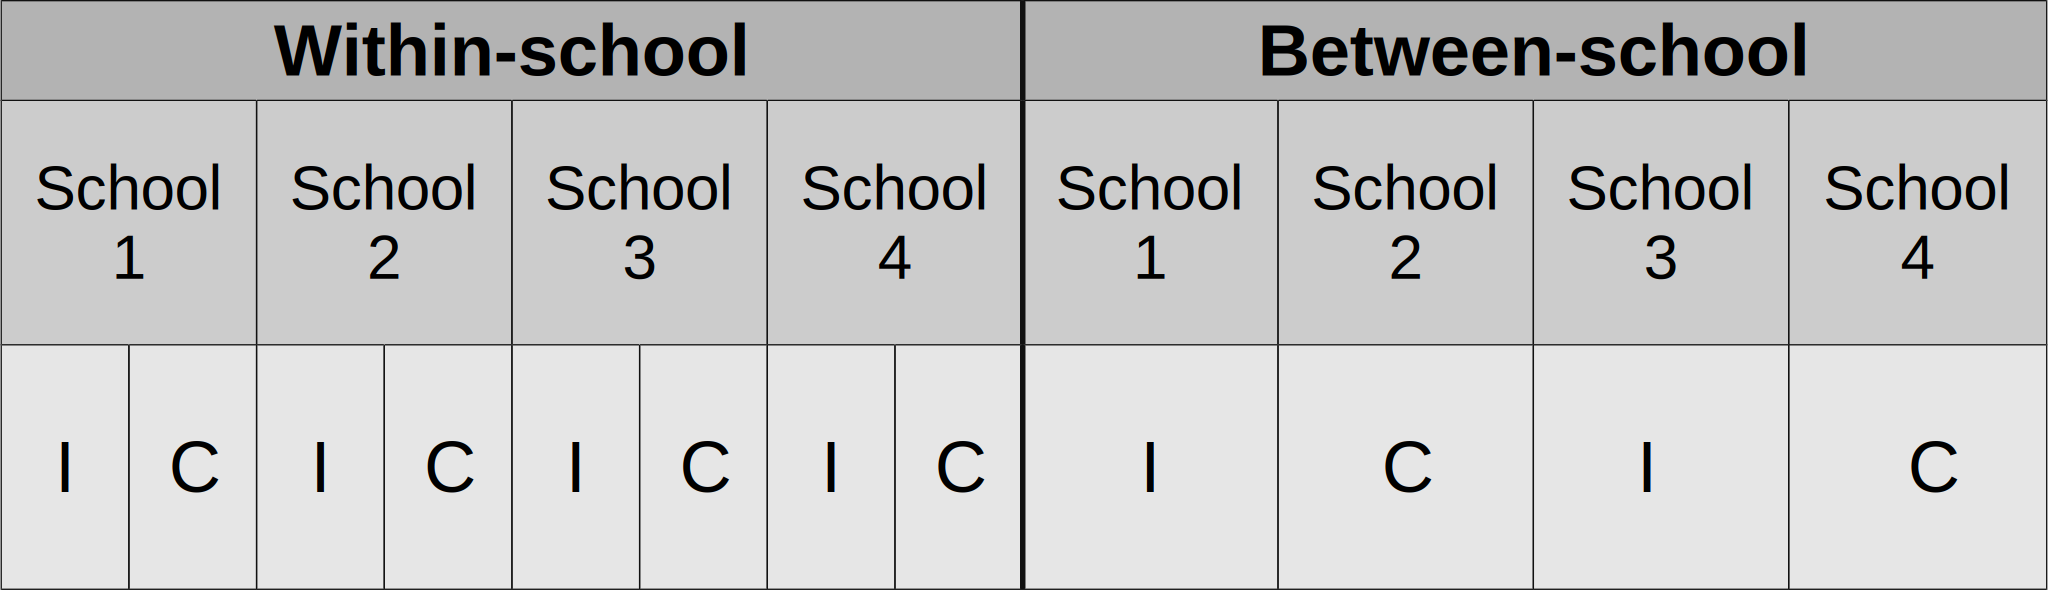
\includegraphics[width=\textwidth]{figure/within_between_school}
  \caption{Within- vs between-school designs. ($I$ for intervention, $C$ for control.)}
  \label{fig:withinschool}
\end{figure}

\begin{description}
 \item[Cluster-randomised design] When clusters are
 assigned in their entiry to the same condition (e.g.,
 all pupils in the same class are assigned to the same
 learning condition rather than each on an individual basis).
\end{description}

\begin{framed}
 In a cluster-randomised design, you need to
 take the cluster-randomisation into account when analysing the data.
\end{framed}

To appreciate the need for taking clustering into account during the analysis, consider an experiment with 6 classes of 10 pupils each. 
There are over one-hundred \emph{quadrillion} ways to split up 60 pupils into two groups of 30 (${60 \choose 30} \approx 1.2 \times 10^{17}$). 
But there are only 20 ways to split up six classes into two groups of three classes each. 
The analysis needs to be based on the assumption that the allocation obtained is one of 20 possible ones, not one of a gazillion ones.

\mypar[Analysis of cluster-randomised designs]{Remark}\label{remark:clusteranalysis}
  One simple and valid approach for analysing data obtained with 
  a cluster-randomised design is to compute the mean (or some other kind of average) 
  of each cluster and then analyse these cluster-level summaries using one of the
  methods covered in Chapter \ref{ch:stats}.
  That said, lots of alternative approaches exist; 
  see \citet{Vanhove2015}, \citet{Vanhove2020c}, and references therein.
\parend

\medskip

% You need to be able to recognise a cluster-randomised design
% and to know that you need to take the cluster-randomisation
% into account during the analysis. But for this class, you don't need to know how to take it
%  into account.\footnote{One simple but valid approach is to compute the mean of each cluster and then analyse these means instead of the raw data.} If you want to conduct an experiment that uses
%  cluster-randomisation, see \citet{Vanhove2015}, \citet{Vanhove2020c}, and references therein.

What you also need to know about cluster-randomisation is this:

 \begin{framed}
   Studies with one intact group as the experimental group and another
   intact group as the control group are useless.
 \end{framed}

 Conceptually, the reason is that class, school and teacher effects can't be separated
 from the effect of the intervention if you just have one intact group
 per condition.
 If you use a rerandomisation test as per Remark \ref{remark:clusteranalysis}
 but you only have a single cluster per group, 
 then there are only two possible allocations.
 As a result, the left- and right-sided $p$-value will both be at least 0.50,
 and the two-sided $p$-value will always be 1.


\mypar{Exercise}
Let's say you want to run a pedagogical experiment (e.g.,
to compare two learning methods for French as a foreign language)
in which randomisation has to take place at the class level rather than at the
individual level.
Other things equal (e.g., number of classes, number of pupils),
what are the advantages and drawbacks of the following designs?
What's the worst option, and why? What's the best, and why?

\begin{enumerate}[(a)]
  \item All classes are taught by the same teacher.
  \item Each class is taught by a different teacher.
  \item One teacher teaches all classes in the control condition,
        and another teacher teaches all classes in the intervention
        condition.
  \item Each teacher teaches two classes: one in the control condition,
        and one in the intervention condition. \parend
\end{enumerate}

\mypar[Reading assignment]{Exercise}
The article by \citet{Slavin2011} makes for pretty challenging reading,
especially in terms of the analysis and the
way the results are presented. But the introductory and methodological sections
discuss some concepts that we've already discussed (especially p.~49).

First try to read the text in full, but skip the parts you find unintelligible.
Then answer the following questions:

\begin{enumerate}[(a)]
  % \item ``[C]hildren's reading proficiency in their native language is a strong \underline{predictor} of their ultimate English reading performance.'' (p.~48, middle, left) What does this mean?
  %
  % \item What do the following terms mean?
  % \begin{enumerate}[i.]
  %   \item matching (p.~49, middle, right)
  %   \item selection bias (p.~49, middle, right, and p.~50, top, left)
  %   \item teacher/school effects (p.~49, bottom, right)
  %   \item within-school design (p.~51, left).
  %         What would the opposite, a between-school design, look like?
  % \end{enumerate}

  \item What is the independent variable in this study?
        What are the dependent variables?

  \item How were the pupils assigned to the different groups?

  \item \citeauthor{Slavin2011} discuss at length how many pupils in each group
  (TBE vs SEI) couldn't be tested (Table 2) and whether the characteristics
  of these pupils differed between the conditions (Table 3). Why do you think
  they discuss this at all?

  \item ``Children were pretested \dots\ on the English Peabody
  Picture Vocabulary Test (PPVT) and its Spanish equivalent, the Test de
  Vocabulario en Imagenes Peabody (TVIP).'' (p.~51, right)
  Why did the researchers go to the bother of conducting such pretests?
  Try to find at least two reasons.

  \item  Comparing Slavin et al.'s Tables 4 and 6,
  we observe that the cohorts' average TVIP
  ({\it Test de Vocabulario en Imagenes Peabody}) scores dropped
  from 99.85 and 90.19 to 92.86 and 85.64, respectively,
  over the course of two years.

  Come up with the most
  plausible explanation for this result.\footnote{Hint: The children's Spanish vocabulary knowledge probably did not
  decline on average as they got older.}\parend
\end{enumerate}

\section{*Examples in R}
See the file \texttt{clusters.html}
in the \texttt{tutorials} directory on \url{https://github.com/janhove/QuantitativeMethodology}.


\chapter{Within-subjects experiments}

\section{Advantages and drawbacks}

Blocking increases power and precision by
pairing up similar participants and randomly assigning one of each pair to
each condition. In within-subjects designs, this idea is taken to an extreme:
the \emph{same} participants are tested in the different conditions.

\medskip

\begin{framed}
In a within-subjects experiment, every participant serves as their own control.
\end{framed}

\medskip

\begin{description}
 \item[Advantage 1: Easier to explore interindividual differences]
 With a between-subjects experiment, you can only estimate
 the average effect of an intervention.
 With a within-subjects experiment, you could additionally gauge
 which participants gain more from an intervention than others.

 \item[Advantage 2: Statistical precision]
 A study's statistical precision depends on
 (a) the amount of data and
 (b) the variability in the data. 
 The \emph{main} (!) advantage of a within-subjects design is that it easily
 accounts for an important source of variability: interindividual differences.
 
 How much more precise a within-subjects experiment is than a
 between-subjects experiment varies from case to case.\footnote{\citet{Quene2010} 
 estimates that within-subjects designs have the statistical precision
 of between-subjects designs with four times as many participants.
 The precise factor depends on the extent to which the participants'
 performance in one condition correlates with their performance in the
 other condition:
 The stronger this correlation, the greater the added value of a
 within-subjects experiment.
 But even if you can't quantify this added value: 
 Within-subjects designs offer more statistical precision.}

 \item[Possible drawback 1: Lack of ecological validity] 
 In applied settings, you typically want the study 
 to mimic the context in which its findings are to be implemented.
 But in such a context, people (e.g., pupils) won't be exposed to several 
 conditions (e.g., learning methods) but rather to just one.
 
 \item[Possible drawback 2: Order and carry-over effects]
 When participants are tested in several conditions,
 it's possible that they learn something in one condition
 that affects their performance in the other condition (\term{carry-over effect}).
 It's also possible that their performance in the last condition differs
 from their performance in the first condition because they've grown
 accustomed to the setting or because they've grown tired of being tested (\term{order effects}).
\end{description}

\section{Minimising order effects}

\begin{description}
 \item[Complete counterbalancing]
 To prevent learning or fatigue effects from exerting a systematic
 effect on the results, you can vary the order of the conditions
 between the participants.
 In complete counterbalancing, \emph{all} possible orders are 
 taken into account. If you have two within-subjects conditions,
 half of the participants first complete condition $A$ and then $B$,
 and the other half first complete condition $B$ and then $A$.
 If you have three conditions, there are $3! = 6$ possible orders;
 you can then randomly assign one sixth of the participants to 
 first complete A, then B, then C;
 one sixth completes A, then C, then B, etc.:
 
\begin{table}[h]
\centering
\caption{Complete counterbalancing for a within-subjects experiment with three conditions.}
\label{tab:counter}
\begin{tabular}{cccccc}
A & A & B & B & C & C \\
B & C & A & C & A & B \\
C & B & C & A & B & A \\
\end{tabular}
\end{table}
\medskip
 
 \item[Latin squares] 
 If a within-subjects experiment has lots of conditions,
 complete counterbalancing is impractical. For four conditions,
 for instance, there are already $4! = 24$ possible orders---we may not
 even have that many participants! The Latin square lends itself
 to such cases.\footnote{`Latin' because the symbols used are typically
 letters of the Latin alphabet.} Latin squares are arrangements of symbols in a grid in which
 each of the symbols used occurs exactly once
 in each row and exactly once in each column. The grid below is a Latin square
 of size 4---one of the 576 possible arrangements of the symbols A, B, C, and D
 that form a Latin square. (Can you come up with a couple of the other 575 ones?)
 
 \begin{table}[h]
\centering
\caption{A Latin square for a within-subjects experiment with four conditions.}
\label{tab:latquad}
\begin{tabular}{cccc}
A & B & C & D \\
B & C & D & A \\
C & D & A & B \\
D & A & B & C \\ 
\end{tabular}
\end{table}
\medskip

  Let's say you picked the Latin square above for your study.
  You'd then randomly assign one quarter of the participants to
  the condition (or stimulus set) order ABCD (first row), 
  one quarter to BCDA (second row),
  one quarter to CDAB (third row) and one quarter to DABC (fourth row).
  The conditions (or stimulus sets) are randomly
  assigned to one of the letters, too.
  
\item[Other possibilities] In which order should we show our
participants 50 pictures that they are to describe if we want to 
prevent order effects from biasing the results?\footnote{Of course,
it's possible that we just accept such `bias' if we aren't interested
in differences between the images, but just in differences between
the participants. If that's the case, these steps may be superfluous.} 
$50! = 3 \cdot 10^{64}$ is an astronomical number,
and even just 50 different Latin square orders seem impractical. One of several
possible solutions is to present the images in a new random order for each participant.
The drawback of doing this is that perhaps image 3 occurs much more often at the start than at the
end of the data collection.
\end{description}

In many psycholinguistic studies, participants need to react
to several stimuli per condition (e.g., 12 stimuli per condition).
The order of the stimuli in these studies are often randomised
so that the conditions are mixed up (e.g., $ABAABBBAB$ etc.).

Counterbalancing and Latin squares don't negate carry-over effects.
Whether carry-over effects represent an acute danger to the study's
validity needs to be judged on a case-by-case basis.
That said, the possible danger of carry-over effects quite often isn't
large enough to offset the certain gain in statistical precision.

\begin{framed}
If you have a genuine choice between a between-subjects
and a within-subjects design for your own research, pick the 
within-subjects design. (Unless, of course, you have an excellent
reason not to do so.)
\end{framed}

\mypar{Example}
  In \citet{Vanhove2018}, I examined the influence of metalinguistic knowledge
  about some structure in the L1 on the participants' intuitions about 
  the corresponding structure in a foreign language.
  Metalinguistic knowledge was manipulated experimentally.
  In the control condition (call it $A$), the participants were 
  given correct but irrelevant information about the L1's morphosyntax.
  In the second condition ($B$), they were given correct, relevant information.
  In the third condition ($C$), they were given correct, relevant information
  and they were additionally taught an algorithm for identifying the structure in question.
  
  It's quite clear that this study couldn't be realised in a within-subjects design:
  Once you give the participants the relevant information (conditions $B$ and $C$), 
  you can't then expect them to suppress this information as they are tested in condition $A$.
  Similarly, once you teach the participants an algorithm for identifying a structure (condition $C$),
  you can't then expect them not to apply it in the other conditions.
  Consequently, I opted for a between-subjects design.
\parend

\mypar{Exercise}
From \citet{Ludke2014}:
 \begin{quote}
Participants were randomly assigned to one of three learning conditions:
speaking, rhythmic speaking, and singing. The participants heard 20 paired-associate
phrases in English and an unfamiliar language (Hungarian) (\dots).
(\dots) The 15-min learning period was followed by a series of five different production,
recall, recognition, and vocabulary tests for the English--Hungarian pairs.
\end{quote}
Re-design this between-subjects experiment as a within-subjects experiment.
What would this description look like? For the time being, ignore the \textit{rhythmic speaking} condition.

In your design, you are constrained by the resources Ludke et al. had. This means that
you cannot introduce stimuli and tests that were not already used by Ludke et al., and
that you have to work with at most 30 men and 30 women as participants.
\parend

\mypar{Exercise}
As in the previous exercise, but with all three conditions.
\parend


\mypar[Reading assignment]{Exercise}
The study by \citet{Kang2013} serves as an example of a within-subjects design. 
Additionally, it uses some turns of phrase commonly found in research reports:

\begin{enumerate}[(a)]
\item ``The Hebrew nouns were learned in one of two training conditions -- retrieval practice or imitation -- that were manipulated within subjects across separate blocks and semantic categories.'' (p.~1261)
\begin{enumerate}[i.]
  \item What does ``manipulated within subjects across separate blocks'' mean?
  \item What does ``manipulated within subjects across semantic categories'' mean?
\end{enumerate}

\item ``The order of items in each test was randomized for each learner.'' (p.~1262) 
        Why?
        Would it have made sense to use the same fixed order of items for all learners?

\item ``In Experiment 2, the order of both tests was counterbalanced across learners\dots'' (p.~1262).
        This merely means that half of the learners first took Test A and then Test B, 
        whereas the other half first took Test B and then Test A.
        Would it have made sense to administer the test in the same order to all learners?\parend
\end{enumerate}

\section{*Analysing data from within-subjects designs with two conditions}
\subsection{AB/BA cross-over design}
  Consider a within-subjects experiment with two conditions, creatively labelled $A$ and $B$, 
  in which participants are randomly assigned to the two possible orders $AB$ and $BA$.
  This design is called a \term{AB/BA cross-over design}.
  We will consider condition $A$ to be the intervention (or treatment) condition
  and $B$ the control condition, but nothing hinges on these labels.
  Let's break down the systematic factors that contribute 
  to the first and second measurements in both orders, see Table \ref{tab:analysiswithin}.
  
\begin{table}[h]
  \centering
  \caption{Systematic factors contributing to the measurements in a within-subjects experiment with two conditions. The meaning of the Greek symbols is explained in the running text.}
  \label{tab:analysiswithin}
  \begin{tabular}{ccc}
    \toprule 
    Order & First measurement & Second measurement \\
    \midrule
    AB    & $\beta + \tau$    & $\beta + \omega + \kappa$ \\
    BA    & $\beta$           & $\beta + \tau + \omega$ \\
    \bottomrule
  \end{tabular}
\end{table}

\begin{itemize}
  \item We assume that there is some baseline $\beta$ common to all measurements.
        This common baseline is of no further interest.
  
  \item There may be treatment effect $\tau$ that contributes to the measurements
        in condition $A$ (i.e., the first measurement for order $AB$ and the second
        for order $BA$), but not to those in condition $B$.\footnote{If there is a treatment effect $\tau'$
        that contributes to the measurements in condition $B$, this is equivalent to there being
        a treatment effect $\tau = -\tau'$ that contributes to the measurements in condition $A$.}
        
  \item There may be an order effect $\omega$ that contributes to the second
        measurements but not to the first measurements.\footnote{Similarly, if an order effect $\omega'$
        contributes to the first measurements instead, write $\omega = -\omega'$.}
        
  \item There may be a carryover effect $\kappa$ that affects the measurements
        in condition $B$ but only if $B$ follows $A$.\footnote{Similarly, if a carryover $\kappa'$ affects
        $A$ when following $B$, write $\kappa = -\kappa'$.}
\end{itemize}

\medskip

In any analysis of these data, 
we need to assume that there are no carryover effects, that is, $\kappa = 0$.
If $\kappa \neq 0$, a within-subjects design was the wrong choice.
Under the assumption that $\kappa = 0$, we may estimate the value of $\tau$ by first computing,
for each participant, the period difference, that is, 
the difference between their first and their second measurement.
For the participants in the $AB$ order, and ignoring any non-systematic effects, we obtain
\[
  d_{AB} = (\beta + \tau) - (\beta + \omega + \kappa) = \tau - \omega - \kappa = \tau - \omega,
\]
since $\kappa = 0$ by assumption.
For the participants in the $BA$ order, we similarly obtain
\[
  d_{BA} = \beta - (\beta + \tau + \omega) = - \tau - \omega.
\]
Observe that
\[
  \frac{d_{AB} - d_{BA}}{2} = \frac{(\tau - \omega) - (- \tau - \omega)}{2} = \tau.
\]
The consequence of this is that, under the assumption of no carryover effects,
the treatment effect $\tau$ can be estimated as half the mean difference in the period
differences between the two orders.
A rerandomisation test or some analytical approximation thereof can be used to obtain a $p$-value for the null hypothesis
that $\tau = 0$.\footnote{In practice, you'll encounter different approaches to analysing within-subjects designs when reading social science studies. Not all of these
are grounded in sound statistical theory.}

\subsection{Interleaved conditions}
Consider again a within-subjects experiment with two conditions, $A$ and $B$,
in which $n$ participants are shown a fixed list of words $w_1, \dots, w_m$.
For each participant, half of the words are shown in condition $A$,
and half are shown in condition $B$;
the presentation software assigns the words to the conditions randomly
and separately for each participant.
The participants react to each word, and their response is expressed numerically
in some fashion (e.g., accuracy, speed, \dots).

For a design like this, there is no real sense in which one condition
follows another condition for each participant.
A sensible way to analyse these data is to compute, for each participant,
the difference score between their average response to condition $A$
and their average response to condition $B$, resulting in difference
scores $d_1, \dots, d_n$.
We then compute the average of these differences, $\overline d$.
Under the null hypothesis of no difference,
each $d_i$ value could just as likely have had the opposite sign.
To generate the distribution of $\overline d$ under the null hypothesis,
we can randomly flip the signs of the observed $d_i$ values
and recompute their average.
Exhaustive sign-flipping would generate the full distribution of $\overline d$
under the null hypothesis, but it involves generating $2^n$ $\overline d$ values.
A Monte Carlo version of this procedure would also work.
Once the distribution of $\overline d$ has been generated or approximated using this sign-flipping,
one- or two-sided $p$-values can be computed as usual.
An analytical short-cut to this procedure is the paired $t$-test on the condition averages per participant.
  
\mypar[Within-school/class designs]{Remark}
  In within-school or within-class designs (see Figure \vref{fig:withinschool}),
  the same procedure can be applied: For each school (or class), compute
  the average score obtained by the pupils in the intervention and the average
  score obtained by the pupils in the control condition.
  Then analyse these averages as described above.
\parend

\section{*Further reading}
Latin-square designs are also used in studies other than 
within-subject experiments, for instance as a technique for blocking.
See \citet{Richardson2018} for an overview and some finer points that weren't discussed here; 
his article is geared towards educational researchers.

\section{*Examples in R}
See the file \texttt{within.html} in the \texttt{tutorials} directory
on \url{https://github.com/janhove/QuantitativeMethodology}.



% LATIN SQUARES ALSO USEFUL FOR BLOCKING. SEE OEHLERT.

% \mypar[Reading assignment]{Exercise}
% The Simon task was (and still is) commonly used in research on any cognitive advantages of bilingualism. In a nutshell, the theory is that bilinguals have to constantly inhibit one of their languages. Because of this, they practice their `inhibitory control'. The Simon task is purported to tap into this same skill (suppressing impulses). As a result, some researchers have interpreted smaller Simon effects in bilinguals as evidence for cognitive advantages of bilingualism. However, these studies have drawn criticism \citep[see the references in][]{Kirk2014}.
% 
% Read pages 640--643 of Kirk et al.\ (2014).
%   Don't read the Results section (it is needlessly complicated),
%   but do take a look at Table 1 and Figure 1.
%   Then answer the following questions; short answers suffice.
%   
%   \begin{enumerate}
%     \item Quasi-experiments tend to be both less conclusive and more arduous
%           than true experiments. Explain why.
%           
%     \item ``Colour assignment to key location was counter-balanced across
%           participants.'' (p.\ 643, top right)
%           Rewrite this sentence without using the word {\it counter-balanced}.
%           Do you have any idea why the researchers effected this counter-balancing?
%           If so, briefly describe it.
%           
%     \item On page 641, the authors make two predictions:
%           \begin{itemize}
%             \item ``If bilingualism, rather than ethnic or cultural background
%             is linked to superior executive control, then both bilingual groups
%             should exhibit an advantage compared to the monolinguals.''
%             
%             \item ``If use of multiple dialects incurs executive control benefits
%             similar to those observed in bilinguals, then differences in executive
%             control between bidialectal monolinguals and bilinguals might be
%             attenuated.''
%           \end{itemize}
%           Do the results in Figure 1 suggest that ``both bilingual groups
%           \dots exhibit an advantage compared to the monolinguals''?
%           Do they suggest that any differences in executive control between
%           bidialectal monolinguals and bilinguals is smaller than 
%           those between non-bidialectal monolinguals and bilinguals?
%           Explain precisely which comparisons you base your answers on.
%           
%     \item Assume you had access to Kirk et al.'s full data set
%           and that you were asked to draw a more informative graph than Figure 1.
%           Draw a sketch of what your graph would look like
%           and briefly explain why your graph is better than Kirk et al.'s.
%           (You do \emph{not} need to draw such a graph in R. A free-hand
%           sketch suffices. Do make sure, however, to indicate clearly
%           what it is that you want to plot. Label your axes.) \parend
% \end{enumerate}          



\chapter{Quasi-experiments and correlational studies}\label{ch:quasi}

Up till now, we've discussed designs that eliminate pre-existing
factors as confounders by means of random allocation or by testing all participants
in all conditions.
We now turn to between-subjects studies without random allocation:
quasi-experiments and correlational studies.

Whether a study counts as a quasi-experiment or a 
correlational study depends on whom you ask.
Some researchers confusingly use the term \textit{quasi-experiment}
to refer to cluster-randomised experiments, whereas others
use the term \textit{pre-experiment} to refer to group comparisons
without randomisation. Similarly, different researchers draw the
border between quasi-experiments and correlational studies at different places.
As far as I'm concerned, the communalities between the two 
outnumber the differences.
For what it's worth, I use the term \term{quasi-experiment} for group comparisons 
and \term{correlational study} when the predictor is continuous.
What's important is that, because no random assignment was used,
we can't assume that the treatment variable is independent of
pre-treatment variables---confounding is a real threat.

\medskip

\begin{description}
  \item[Quasi-experiment] Group comparison, but the groups weren't constructed using random assignment.
  \begin{itemize}
   \item Example 1: Comparison of pupils with and
      without an immigration background.
   \item Example 2: Comparison of children that take
      heritage language classes and children that don't.
  \end{itemize}

  It doesn't matter whether the groups \emph{could} have
  been constructed using random assignment, just whether they were.

  \item[Correlational study] No group comparison.
  Instead, one assesses to what extent variation in
    an outcome (dependent) variable can be accounted
    for by differences in one or more continuous predictors (independent variables).
    The values of these predictors weren't assigned to the units of observation
    randomly.

  \begin{itemize}
   \item Example 1: Researchers collect IQ and
    L2 proficiency data in a group of learners and
    assess how strongly both types of data covary.

   \item Example 2: Using archival data,
    researchers gauge how well they can account for whether
      children will pass their A-levels based on the results of a
      vocabulary test when the children were 12 years old.
  \end{itemize}
\end{description}

\paragraph{Why carry out quasi-experiments and correlational studies?}

 \begin{quote}
``But just because full experimental control \emph{is} lacking, it becomes imperative that the researcher
\textbf{be thoroughly aware of which specific variables his particular design fails to control}.

``The average student or potential researcher reading the previous section of this chapter probably ends up with more things to worry about in designing an experiment that he had in mind to begin with.
This is all to the good if it leads to the \textbf{design and execution of better experiments and to more
circumspection in drawing inferences from the results}.
It is, however, an unwanted side effect if it creates a feeling of hopelessness with regard to achieving
experimental control and leads to the abandonment of such efforts in favor
of even more informal methods of investigation.

``[W]e shall \dots survey the strenghts and weaknesses of a heterogeneous collection of quasi-experimental designs, each deemed worthy of use \emph{where better designs are not feasible}.'' \citep[p.~34; their emphasis in italics, mine in bold-face]{Campbell1963}
\end{quote}

\medskip

The goal of quasi-experiments and correlational studies
is often to draw causal conclusions, but the findings---for better
or for worse---tend to be couched in non-causal language \citep{Grosz2020}.

\mypar[Controlling for confounds is difficult]{Exercise}
Consider the following description:

\medskip

\begin{quote}
``There were 40 participants who composed two language groups and two age groups.
Twenty of the participants were younger adults ranging in age from 30 to 54
years (mean age = 43.0 years), and 20 were older adults ranging in age from
60 to 88 years (mean age = 71.9 years). In each age group, half the participants
were monolingual English speakers living in Canada, and the other half were
Tamil--English bilinguals living in India. (\dots) All the participants in
both groups had bachelor's degrees \dots'' \citep[p.~44]{Bialystok2004}
\end{quote}

\medskip

While the authors didn't explicitly claim to have done so,
you might end up thinking that level of education was controlled
for in this study. A couple of minutes' thought should reveal
that this wasn't the case. (Does having a minimum requirement
of having Bachelor's degrees equate both groups with respect
to level of education?) But more interestingly, by introducing
this minimum requirement, the authors may have introduced
\emph{additional} bias.
How so?\footnote{If you're stuck, consult \url{https://gpseducation.oecd.org/CountryProfile?primaryCountry=CAN&treshold=5&topic=EO} and look up similar data for India.}\parend

\section{Correlation coefficients}
\term{Pearson correlation coefficients}, typically just called
correlation coefficients and abbreviated as $r$,
express how closely the ($X$,$Y$) data points fall on a straight line.

\begin{itemize}
 \item $r = 1$: All points fall exactly on an increasing line.
 \item $r = -1$: All points fall exactly on a decreasing line.
 Correlation coefficients of $1$ or $-1$ (or close to it, e.g., $r = 0.99$)
 tend not to be too interesting: They typically indicate that the two variables
 express the same thing (e.g., body length in centimetres and in inches).
 \item $r = 0$: There's no linear relation between the two variables whatsoever.
\end{itemize}

Correlation coefficients work in both directions: $r_{XY} = r_{YX}$.

Figure \ref{fig:correlations} shows eight examples of scatterplots
and the correlation coefficients for the data presented in them.
Note that a correlation coefficient close to zero doesn't imply
that there is no relation between them;
correlation coefficients different from 1 or -1 don't imply that
the relation between two variables is imperfect;
and it's possible for a positive correlation coefficient to reflect
a relationship that's largely negative, and vice versa.
Do these examples contradict the rough definition of correlation coefficients
given above?



\begin{figure}[tpbh]
  \centering
  \includegraphics[max width = \textwidth]{figure/correlations-1}
  \caption{Examples of scatterplots and their associated correlation coefficients.}
  \label{fig:correlations}
\end{figure}

\begin{framed}
The same correlation coefficient can correspond to a multitude of relationships
between two variables.
Never \emph{ever} compute a correlation coefficient without drawing a scatterplot first.
\end{framed}

\medskip

By the same token, don't put stock in conclusions that hinge crucially on
correlation coefficients for which no scatterplots are provided.

\mypar[Honing intuitions about correlation coefficients]{Exercise}
To hone your intuitions about correlation coefficients, you can use
the \texttt{plot\_r()} function from the \texttt{cannonball} package
for \texttt{R}.\footnote{If you run into the error message `Failed to install `unknown package' from GitHub', try running the command \texttt{Sys.unsetenv("GITHUB\_PAT")} first.}

\begin{knitrout}
\definecolor{shadecolor}{rgb}{0.969, 0.969, 0.969}\color{fgcolor}\begin{kframe}
\begin{alltt}
\hlcom{# Install the package}
\hlkwd{install.packages}\hldef{(}\hlsng{"devtools"}\hldef{)}
\hldef{devtools}\hlopt{::}\hlkwd{install_github}\hldef{(}\hlsng{"janhove/cannonball"}\hldef{)}

\hlcom{# Load the functions}
\hlkwd{library}\hldef{(cannonball)}

\hlcom{# Draw 16 plots with 20 data points each and r = 0.6}
\hlkwd{plot_r}\hldef{(}\hlkwc{n} \hldef{=} \hlnum{20}\hldef{,} \hlkwc{r} \hldef{=} \hlnum{0.6}\hldef{)}

\hlcom{# With 50 data points each and r = 0.0}
\hlkwd{plot_r}\hldef{(}\hlkwc{n} \hldef{=} \hlnum{50}\hldef{,} \hlkwc{r} \hldef{=} \hlnum{0.0}\hldef{)}

\hlcom{# With 40 data points and r = -0.9}
\hlkwd{plot_r}\hldef{(}\hlkwc{n} \hldef{=} \hlnum{40}\hldef{,} \hlkwc{r} \hldef{=} \hlopt{-}\hlnum{0.9}\hldef{)}
\end{alltt}
\end{kframe}
\end{knitrout}

Type \texttt{?plot\_r} at the R prompt to access the function's
help page and read the text under `Details'.\parend

\section{Statistical control using hierarchical regression}

\mypar[Reading assignment]{Exercise}
The next reading assignment concerns the study by \citet{Slevc2006}.
The ```zero-order correlations'' mentioned
are correlation coefficients expressing the relationship between two measured variables.
(``First-order correlations'' would be correlation coefficients expressing the relationship between two variables from which the influence of a third variable was statistically `partialled out'.)

To help you make sense of Table 3:
\begin{itemize}
 \item $R^2$: The proportion of the variation (`variance') in the outcome variable that can be described using the predictor
 variables included in the regression model.

 \item $\Delta R^2$: The increase in $R^2$ compared to the previous \textit{step} (i.e., the improvement in $R^2$ attributable to the current predictor).

 \item \textit{df}, $F$: You can ignore this for this class.

 \item \textit{Final $\beta$}: Expresses the form of the relationship between the predictor in question and the outcome.
\end{itemize}

\medskip

Now to the questions:
\begin{enumerate}[(a)]
  \item What was the most important goal that \citet{Slevc2006} set themselves?

  \item Why did they have this aim?

  \item Why did they collected the variables \textit{age of arrival},
  \textit{length of residence}, \textit{language use and exposure}
  and \textit{phonological short-term memory}?

  \item Which conclusions do they draw on the basis of their results?

  \item Regardless of whether you agree with these conclusions: Try
  to find one or two alternative explanations for their results
  that call into question the claim that ``musical skills may
  facilitate the acquisition of L2 sound structure'' (abstract).\parend
\end{enumerate}

\medskip

In correlational studies, control variables are often used to
adjust statistically for known confounders.
One technique used to accomplish this is hierarchical regression;
see Table 3 in \citet{Slevc2006} for an example.
We will discuss this technique mainly so that you
are better able to appreciate the shortcomings of this
technique and ones similar to it.

\paragraph{Example}
If you measure the shoe size and vocabulary knowledge of 4- to 16-year-olds,
you'll observe a positive correlation between the two. This isn't surprising;
see Figure \ref{fig:shoe}.
We'll use this silly example to illustrate the principle behind
hierarchical regression; see Figure \vref{fig:hierarchical}.

\begin{marginfigure}
  \includegraphics{figure/shoe}
  \caption{Shoe size and vocabulary knowledge are correlated since age
  acts as a confound.}
  \label{fig:shoe}
\end{marginfigure}

\begin{itemize}
 \item Top left: Shoe size and vocabulary knowledge are positively correlated.

 \item Top right and middle left: Age---the confound---is correlated
 positively with both shoe size and vocabulary knowledge.

 \item Middle right: This plot shows the vertical distance between
 the points in the middle left panel and the regression line.
 This shows how much the participants vary in their vocabulary
 test scores once the linear association between age and vocabulary
 knowledge has been partialled out.

 \item Bottom left: The association between shoe size and the vocabulary
 test scores with the linear association of age partialled out is much
 less strong. In this simulated example, the fact that the remaining
 association isn't exactly zero is due entirely to chance.
\end{itemize}




\begin{figure}[tpbh]
  \centering
  \includegraphics[max width = \textwidth]{figure/hierarchical-1}
  \caption{Hierarchical regression used to control for the age confound in the relationship between shoe size and vocabulary knowledge. The coloured circles in each panel show data belonging to the same three participants. The straight lines are regression lines. A regression line is the straight line that best captures the tendency in the cloud of data points, according to some definition of `best'.}
  \label{fig:hierarchical}
\end{figure}

\clearpage

\section{Caveats}
You need to be hyper-aware of the following caveats
concerning statistical control:

\begin{enumerate}
  \item Controlling for a number of possible confounds doesn't rule
  out the possibility that there are even more confounds; Figure \ref{fig:caveat1}.

  \begin{marginfigure}
    \centering
    \includegraphics{figure/caveat1}
    \caption{Perfectly controlling for $A$ and $B$ closes the non-causal paths $X \leftarrow A \rightarrow Y$ and $X \leftarrow B \rightarrow Y$. But it leaves open the non-causal path via $U$.}
    \label{fig:caveat1}
  \end{marginfigure}

  \item The methods typically used to account for confounding variables
  account for \emph{linear} relationships between the confounds and the
  variables of interest. If these relationships aren't linear, the
  confound won't be fully accounted for. In \textsc{dag} parlance, the path
  via the confound won't be fully closed.

  \item The `confound' may be a post-treatment variable. See Section
  \vref{sec:covariates}.

  \item Statistical control may be imperfect because the confound was
  measured with some error. We'll treat this in more detail in Chapter
  \ref{ch:measurementerror}.

\end{enumerate}

\medskip

The following excerpt makes the same points:
\begin{quote}
``When experimental designs are premature, impractical, or impossible,
researchers must rely on statistical methods to
adjust for potentially confounding effects.
Such procedures, however, are quite fallible.
We examine several errors that often follow the use of statistical adjustment.

``The first is inferring a factor is causal because
it predicts an outcome even after ``statistical control''
for other factors. This inference is fallacious when (as usual) such control
involves removing the linear contribution of
imperfectly measured variables, or when
some confounders remain unmeasured.

``The converse fallacy is inferring a factor is not causally
important because its association with the outcome is attenuated
or eliminated by the inclusion of covariates in the adjustment
process. This attenuation may only reflect that the covariates treated as
confounders are actually mediators (intermediates) and
critical to the causal chain from the study factor to the study
outcome.\footnote{What's meant is a causal chain such as $A \rightarrow B \rightarrow C$.
$A$ is causally important, but if you control for $B$, you won't find
any association between $A$ and $C$.}

``Other problems arise due to mismeasurement of the study factor or outcome,
or because these study variables are only proxies for underlying constructs.

``\emph{Statistical adjustment serves a useful
function, but it cannot transform observational studies into natural experiments, and involves far more subjective judgment than
many users realize.}''
\citep[abstract, my emphasis]{Christenfeld2004}
\end{quote}

\medskip

\begin{framed}
Large sample sizes don't solve these problems.
\end{framed}

\medskip
Also see the blog entry \href{https://janhove.github.io/posts/2015-08-24-caveats-confounds-correlational-designs/}{\textit{Controlling for confounding variables in correlational research: Four caveats}}.

\mypar{Exercise}
In this series of exercises, we will use R to simulate some data
  and perform correlation analyses on them. More concretely, we will generate
  $n = 200$ pairs of predictor--outcome observations. The predictor $\bm x = (x_1, \dots, x_n)$
  will be sampled from a normal distribution with mean 0 and variance 1
  (i.e., $x_i \sim \mathcal{N}(0, 1)$).
  The outcome $\bm y$ is described by a simple function of $\bm x$ and some random error,
  namely,
  \[
    y_i = 0.4 + 0.7 \cdot x_i + \varepsilon_i,
  \]
  $i = 1, \dots, n$, where the random error $\bm \varepsilon = (\varepsilon_1, \dots, \varepsilon_n)$
  is also sampled from a normal distribution with mean 0 and variance 1
  (i.e., $\varepsilon_i \sim \mathcal{N}(0, 1)$),
  independently of both $\bm x$ and the other $\varepsilon_i$ values.

  Run the following commands in R to simulate data according to this scheme.
Note that the \texttt{rnorm()} command takes an argument that specifies the standard
  deviation (\texttt{sd}) of the normal distribution from which to sample the data,
  not its variance. But since $\sqrt{1} = 1$, the standard deviation of the
  distribution from which we sample is also 1.
  (Like for the graphing assignments, don't enter these commands directly to the console. Use a script.)

\begin{knitrout}
\definecolor{shadecolor}{rgb}{0.969, 0.969, 0.969}\color{fgcolor}\begin{kframe}
\begin{alltt}
\hldef{n} \hlkwb{<-} \hlnum{200}
\hldef{x} \hlkwb{<-} \hlkwd{rnorm}\hldef{(n,} \hlkwc{mean} \hldef{=} \hlnum{0}\hldef{,} \hlkwc{sd} \hldef{=} \hlnum{1}\hldef{)}
\hldef{y} \hlkwb{<-} \hlnum{0.4} \hlopt{+} \hlnum{0.7} \hlopt{*} \hldef{x} \hlopt{+} \hlkwd{rnorm}\hldef{(n,} \hlkwc{mean} \hldef{=} \hlnum{0}\hldef{,} \hlkwc{sd} \hldef{=} \hlnum{1}\hldef{)}
\end{alltt}
\end{kframe}
\end{knitrout}
  The expected correlation between $\bm x$ and $\bm y$ is
  \begin{align*}
    \rho_{xy} 
    &= \frac{0.7 \cdot \textrm{Var}(\bm x)}{\sqrt{\textrm{Var}(\bm x)(0.7^2 \cdot \textrm{Var}(\bm x) + \textrm{Var}(\bm \varepsilon))}} \\
    &= \frac{0.7}{\sqrt{0.7^2 + 1}} \\
    &\approx 0.57,
  \end{align*}
  since $\textrm{Var}(\bm x) = 1 = \textrm{Var}(\bm \varepsilon)$.

  We now put these $\bm x, \bm y$ observations into a tibble.

\begin{knitrout}
\definecolor{shadecolor}{rgb}{0.969, 0.969, 0.969}\color{fgcolor}\begin{kframe}
\begin{alltt}
\hlkwd{library}\hldef{(tidyverse)}
\hldef{d} \hlkwb{<-} \hlkwd{tibble}\hldef{(}\hlkwc{predictor} \hldef{= x,} \hlkwc{outcome} \hldef{= y)}
\end{alltt}
\end{kframe}
\end{knitrout}

  \begin{enumerate}
    \item Using \texttt{ggplot()}, draw a scatterplot of the \texttt{predictor}
    vs.\ \texttt{outcome} values in \texttt{d}.

    \item Compute the sample correlation coefficient between \texttt{predictor}
    and \texttt{outcome} using the R function \texttt{cor()} like so:
\begin{knitrout}
\definecolor{shadecolor}{rgb}{0.969, 0.969, 0.969}\color{fgcolor}\begin{kframe}
\begin{alltt}
\hlkwd{cor}\hldef{(d}\hlopt{$}\hldef{outcome, d}\hlopt{$}\hldef{predictor)}
\end{alltt}
\end{kframe}
\end{knitrout}
    Jot down this number, rounded to two decimal places.
    Now simulate the data again and jot down the number again; do this five times.
    Compare the correlation coefficients you observed to the expected correlation coefficient
    and summarise your findings.

    \item Now imagine that instead of observing a random sample of $n$ observations,
    we only observe data from those pairs of observations where $x_i > 0$.
    To emulate this scenario, we create a new tibble (\texttt{d2}) consisting of those rows
    in \texttt{d} where the predictor value is greater than 0:
\begin{knitrout}
\definecolor{shadecolor}{rgb}{0.969, 0.969, 0.969}\color{fgcolor}\begin{kframe}
\begin{alltt}
\hldef{d2} \hlkwb{<-} \hldef{d |>}
  \hlkwd{filter}\hldef{(predictor} \hlopt{>} \hlnum{0}\hldef{)}
\end{alltt}
\end{kframe}
\end{knitrout}

    Draw a scatterplot of the \texttt{predictor}
    vs.\ \texttt{outcome} values in \texttt{d2}.
    Compute the sample correlation coefficient between \texttt{predictor}
    and \texttt{outcome} in this reduced sample.
    Repeat the entire simulation five times.
    Compare the correlation coefficients you observed to the expected correlation coefficient
    and summarise your findings.

    \item Now imagine that instead of observing a random sample of $n$ observations,
    we only observe data from those pairs of observations where $x_i > 1$ or
    where $x_i < -1$; equivalently, where $|x_i| > 1$. That is, we're only retaining
    data with fairly extreme $x_i$ observations.

    Using \texttt{filter()}, create a new tibble (\texttt{d3}) consisting
    of those rows in \texttt{d} where the absolute predictor value is greater than 0.
    You can use the \texttt{abs()} function to compute absolute values.

    Draw a scatterplot of the \texttt{predictor}
    vs.\ \texttt{outcome} values in \texttt{d3}.
    Compute the sample correlation coefficient between \texttt{predictor}
    and \texttt{outcome} in this reduced sample.
    Repeat the entire simulation five times.
    Compare the correlation coefficients you observed to the expected correlation coefficient
    and summarise your findings.\parend
  \end{enumerate}


\chapter{Constructs and indicators}\label{ch:measurementerror}

We're faced with an inescapable fact of life:

\medskip

\begin{framed}
Most measurements are imperfect.
\end{framed}

\medskip

Saying that a study's measurements aren't perfect isn't much of a criticism.
But it's crucial to appreciate the consequences of imperfect measures---pointing
out that a study's findings can plausibly be accounted for by the fact
that its measurements are imperfect \emph{is} a valid criticism.

\medskip

\begin{description}
  \item[Construct] or \textit{latent variable}. 
  Lots of characteristics can't be observed or measured directly.
  Instead, their existence, as well as their relative value, are
  inferred on the basis of other, observable variables.
  
  \item[Indicator] or \textit{manifest variable}. 
  These are variables that can be measured or observed directly
  and from which information about the construct is inferred.
  Table \vref{tab:constructs} lists some examples.
  
\begin{table}
\centering
\begin{tabular}{p{4.75cm}p{5cm}}
  \toprule
  Construct                               &   Example indicator \\
  \midrule  
  Intelligence                            &   Result on an intelligence test\\
  Working memory capacity                 &   Length of a sequence of digits you can repeat in reversed order\\
  Language aptitude                       &   Result on the LLAMA-D test\\
  L2 reading skills                       &   Number of correctly answered items on a reading test\\
  Attitudes towards Danish                &   Answer to the question `How beautiful do you think Danish is?'\\
  Socio-economic status                   &   Father's occupational category\\
  \bottomrule
\end{tabular}
\caption{Examples of constructs and indicators.}
\label{tab:constructs}
\end{table}

  \item[Measurement error] Even the best indicators are rarely perfect.
  Better indicators just have a smaller measurement error.
  
  Even variables that don't act as proxies for some cognitive or social
  construct are often measured with some error. Examples include
  body weight (bathroom scales are imperfect, and the result is rounded),
  blood pressure (if you have a sphygmomanometer, 
  check its manual),
  and age (invariably rounded down to the integer below when reported).
\end{description}

\section{Systematic and random measurement error}
Measurement error can include both a systematic and a random component.

The \term{systematic} component of an instrument's measurement error is the extent
to which it tends to over- or underestimate what it's supposed to measure.
For instance, a miscalibrated kitchen scale may overestimate weights by 10 g on average,
and an overly harsh language test may tend to label learners' L2 skills
one CEFR level below their actual proficiency on average.

Note that it's possible for an instrument to systematically overestimate
values on one part of the scale and to underestimate them on another part.

When there's no gold standard to which the measurements can be compared,
it may be impossible to assess their systematic measurement error.

The \term{random} component of an instrument's measurement error is the
extent to which the measured values differ from the true values + 
systematic error.
Another way of putting this is: By how much will the
measurements vary if the true values are the same?
For instance, an kitchen scale may, on average, measure weights
accurately (no systematic error), 
but the individual readings may be off by up to a couple of grams 
in either direction (random error).

As a second example, consider a group of 365 7-year-olds, all born
on different days of the year. Just one of them actually is 7 years old
on the day; the reported values of the others will be off by 1 day, 2 days, \dots,
364 days. The reported age, then, systematically underestimates their true age
by $\frac{0+1+2+\dots+364}{365} = 182$ days.
The random component is 0, though, as children born on the same day will report
the same age, even though this reported age will be lower than their actual age.

As a final example, consider a poorly calibrated bathroom scale. If you put
a calibrated mass of precisely 60 kg on it on five different occassions, it returns
readings of 61.1, 60.4, 60.4, 60.5 and 61.2.
The mean observation for the same mass is $\frac{61.1+60.4+60.4+60.5+61.2}{5} = 60.78$,
i.e., an overestimate of 0.78 kg.
The mean absolute difference between the observations and their expected
value (here: 60.78) is $\frac{|0.32| + |-0.38| + |-0.38| + |-0.28| + |0.72|}{5} = 0.42$.

\section{Consequences of measurement error}

The consequence of systematic measurement error is clear: Your data are biased.
This isn't necessarily a problem: If you're comparing two groups for both
of which you have data that are biased to the same extent, the difference between
them won't be biased. And for variables such as age, the systematic error (roughly
182 days) tends to be small relative to the variability of the true values, in 
which case it's probably inconsequential.\footnote{But see, for instance, 
\citet{Helsen2005} and \citet{Sprietsma2010} on the consequences of `relative age' (i.e., age 
differences within an age group, e.g., 15-year-olds) in sports and education.}

The consequences of random measurement error are much less intuitive and bear
pointing out.

\paragraph{Less power and precision}
Measurement error on the \emph{outcome} variable will increase
its variability. Since power and precision are lower when
there's more variability in the outcome, 
measurement error on the outcome lowers power and precision.

\paragraph{Statistical control is imperfect}
Measurement error on a \emph{control} variable means that 
controlling for this observed variable won't fully eradicate 
the confounding caused by the construct itself.
The \textsc{dag} in Figure \ref{fig:caveat2} illustrates this.

\begin{marginfigure}
  \centering
  \includegraphics{figure/caveat2}
  \caption{The $X$--$Y$ relationship is confounded by $A$. $A$, however,
  can't be observed directly. A proxy (indicator) $A_{obs}$ can be controlled for instead, but this won't fully shut the non-causal path $X \leftarrow A \rightarrow Y$.}
  \label{fig:caveat2}
\end{marginfigure}

\begin{quote}
``[F]allibility in a covariate usually implies that there would be more adjustment if the variable were measured without error.'' \citep[p.~569]{Huitema2011}
\end{quote}
  
Controlling for $A_{obs}$ is better than not controlling for it.
But researchers routinely mistake 
controlling for an indicator with controlling for a construct,
and their causal conclusions are overconfident as a result.
A discussion of this problem can be found in
\citet{Westfall2016}, \citet{Vanhove_HELASCOT_results}
and \citet{Berthele2017b}.

\paragraph{Regression to the mean}
When observations are due partly to skill or some underlying
construct and partly to chance (e.g., measurement error), 
a second round of observations will likely show that the 
extreme scores have become less extreme, i.e., that they've regressed
to the mean.

\begin{itemize}
\item First consider an example where the observations are purely due to luck,
with no skill or construct involved: playing roulette. Playing roulette
is a losing proposition: For every 100 francs bet, you stand to lose about 5
francs (= the mean). But on any given night, some players will luck out and
make a killing, whereas other players get extraordinarily unlucky and lose much
more than the expected 5 francs. Their winnings or losses are a dreadful measure
of their skill level: they all have the same skill level, which corresponds
to a loss of 5 francs.

The next night, however, the lucky players from the
day before probably won't get as lucky again (their luck the day before was
extraordinary), and similarly for the unlucky players---all again stand to
lose about 5 francs. Some might get lucky or unlucky twice in a
row, but they're more likely to end up somewhere near the 5-franc mark, i.e., most
of the lucky and unlucky players will regress to the mean.

\item The same principle is at play when the observations come about in part through
skill (or some other construct) and in part through chance.
For instance, the most successful stock picker of the year 2032 is likely
 not to perform as well in the year 2033---even if the conditions
 on the stock market are comparable and the stock picker didn't start to 
 rest on his laurels. The reason could simply be that he had more
 than his fair share of luck in 2032---you need some luck to 
 come out on top---and wasn't as lucky in 2033. As a result,
 his performance in the next year is likely to be closer to the
 average performance (i.e., he's regressed to the mean of stock
 picker performance).
 
 \item If you administer a reading test to a group of learners
 one week and another reading test a couple of weeks later,
 you're likely to find that the very worst readers on the first test
 are still pretty poor readers on the second test (= the skill part),
 but their performance won't be as atrocious---it'll seem as though
 they've made some progress. Similarly, the best readers on the first
 test are likely to still be good readers on the second test, but
 their performance probably won't be as exceptional---it'll seem as
 though they've become worse.
 
 But this pattern can be explained in
 terms of measurement error: Even if none of the learners actually
 learnt or unlearnt something, you're likely to find such a pattern.
 The reason is that, if you obtained a dismal score, you're likely
 to be a pretty poor reader \emph{and} to have had some bad luck---perhaps
 the topic of the reading test just wasn't suited for you, or you
 were coming down with the flu. A couple of weeks later, you might
 encounter a topic you know a thing or two about or you might
 be in better physical shape.
 Similarly, if you scored exceptionally well on the first test,
 you may have had some luck with the test's topic or with other
 circumstances, and these may not be as favourable next time round.
\end{itemize}

\mypar{Exercise}
A nationwide standardised maths test is administered
to all 5th graders. It turns out that the classes with
the highest mean test scores tend to be pretty small.
One possible explanation is that small classes are more
conducive to learning maths.
Another explanation is that this finding is an artefact
of measurement error. 
These explanations aren't mutually exclusive.

\begin{enumerate}[(a)]
  \item Explain how measurement error can give rise to this finding.
  \item How could you check if measurement error accounts (fully or in part)
        for this finding?\footnote{Hint: Which graph could you draw?}\parend
\end{enumerate}


\chapter{Questionable research practices}

\mypar[Reading assignment]{Exercise}
Read Chapter 2 in \citet{Chambers2017}.
There are no guiding questions for this text; it should be
intelligible enough. But by way of preparing for it, try
to answer these questions.

\begin{enumerate}[(a)]
  \item You recruit 60 participants, aged 8--88. Half of them
  are assigned to the experimental group; the others to the
  control group (random assignment). You run a significance test
  comparing the mean age in both groups. What is, at most, the probability
  that you'll obtain a significant result (i.e., $p \leq 0.05$)?
  
  \item Each of your participants throws a fair six-sided dice.
  You run another significance test to check if there's a mean
  difference in the number of pips obtain in the control and in
  the intervention groups. (Evidently, the intervention doesn't
  make you throw dice any better.)
  What is, at most, the probability
  that you'll obtain a significant result (i.e., $p \leq 0.05$)?
  
  \item What do you know about the probability of observing
  \emph{either} a significant age difference between the two groups,
  \emph{or} a significant difference in the mean number of pips obtained,
  \emph{or} two significant differences? \parend
\end{enumerate}

\section{A paradox}
\citet{Sterling1995} inspected 563 articles in psychology
journals (published in 1986--1987) in which significance tests
were used to answer the research question.
In 538 of them (96\%), the researchers reported a significant
result that confirmed their own hypothesis.
In medical journals, the figure was lower but still pretty high
(270/316, 85\%).

\begin{figure*}
\centering
\includegraphics[width=\textwidth]{figure/Sterling1995}
\caption{Table 1 from \citet{Sterling1995}.}
\label{fig:sterling}
\end{figure*}

But at the same time, the sample sizes in psychological research
are fairly small \citep{Marszalek2011,Sedlmeier1989}: The average
study in applied psychology published in 1995 only contained 
22 participants per condition. This implies that many of these studies
must have had fairly low statistical power (see Section \vref{sec:power}): 
Even if the null hypothesis hadn't been correct in any of these studies,
it'd have been impossible to reject it in 96\% of cases.

For a long time \citep[see already][]{Sterling1959}, it was believed
that the reason for this discrepancy (low power, lots of significant
results) was due to \term{publication bias}: 
Researchers prefer to write up the studies in which they obtained
significant results, and editors and reviewers tend to reject
studies with non-significant findings. The studies that were conducted
but that produced non-significant findings were believed to languish
in the researchers' file-drawers.

But while some studies never make it into print, the vast majority do.
So where did the non-significant findings go?

\section{Hidden flexibility}

More recently, scholars with an interest in meta-science (i.e.,
science about science) have come to realise that research projects
afford a great deal of flexibility. Researchers can---consciously
or subconsciously---leverage this flexibility to produce a steady stream
of significant findings---\emph{even if the data are nothing but noise}.\footnote{If the data aren't just noise, such flexibility will spuriously amplify the signal. For instance, even if $A$ influences $B$, the literature as a whole will tend to overestimate the extent of this influence.}\\
\citet{Simmons2011} call this flexibility \term{researcher degrees of freedom} 
and demonstrate how significant findings can be 
conjured from thin air if researchers afford themselves some leeway in
analysing their data.

Sources of researcher degrees of freedom include:

\begin{itemize}
  \item A researcher can run intermediate analyses 
  and decide to stop or to continue collecing data based on the results. 
  See \citet{Simmons2011} and Exercise \ref{ex:fpp} for the consequences of this.
  
  \item Sometimes, there are several ways in which a task or test can be
  scored, or how some variable can be constructed.
  When one way yields a significant finding and the other doesn't,
  it's easy to convince yourself that the one that produced significance
  was obviously the right one. 
  Relatedly, researchers routinely collect multiple outcome variables, but
  it's tempting to focus on the one that `worked' (i.e., produced significance)
  rather than on those that didn't.
  See \citet{Simmons2011},
  \citet{Gelman2013}, and 
  \citet{Malsburg2017}. For a discussion with a focus on bilingualism
  research, see \citet{Poarch2018}.
  
  \item \term{HARKing} \citep[hypothesizing after the results are known;][]{Kerr1998}: 
  A largely exploratory analysis is reported as though it were planned all along.
  Inevitably, the researchers will find in the data what they claim to have
  anticipated. (This can happen without any bad intent on the part of the
  researchers.)
  
  \item Convenient errors and biased debugging: 
  Everyone makes mistakes, but you're more likely to catch your own
  mistakes when the results don't pan out than when they do.
  As a result, the mistakes that remain in the literature aren't
  distributed randomly but tend to favour the researchers' hypotheses.
  
\end{itemize}

Trying out several defensible analyses and glossing over the ones
that didn't produce significance is referred to as \term{p-hacking}.

The practices listed above are examples of questionable research practices.
Traditionally, these aren't viewed as outright fraud (which includes 
fabricating or manipulating data), though arguably, it will become increasingly
difficult to invoke plausible deniability 
as professional researchers can be expected to know their consequences.

For possible solutions, see \citet{Chambers2017}.

\mypar[False-positive psychology]{Exercise}\label{ex:fpp}
The consequences of researcher degrees of freedom/p-hacking are
best appreciated by seeing them. Do these exercises in order.

\begin{enumerate}[(a)]
  \item Open the app at \url{https://plurilinguisme.shinyapps.io/fppsy/}
  and carefully read the description.
  
  \item Click `Simulate!', leaving all settings at their default values.
  Describe what the two graphs (reproduced here as Figure \ref{fig:app} for your convenience) are showing.
  
\begin{figure}
\centering
\includegraphics[width=\textwidth]{figure/app}
\caption{When you run the app using its default settings, you'll obtain two graphs similar to these. Your graphs won't be identical as they are based on simulations with random data.}
\label{fig:app}
\end{figure}
  
  \item First try to answer the following questions by \emph{thinking}
  about them. Once you've written down your answer, check it by
  running the simulation.
  
  \begin{enumerate}[i.]
    \item Increase the `maximum number of additional participants in each group' to 30. Leave the other settings at their default values. How will the graphs change?
    
    \item Leaving all other settings as they currently are, what will
    happen if instead of analysing the data after 10 new participants
    per condition, they're analysed after 5 new participants per
    condition? Or after just 2 new participants per condition?
    
    \item What'll happen when the correlation between the two 
    dependent variables becomes weaker (e.g., $r = 0.1$ instead
    of $r = 0.5$)? Why?
    
    \item What'll happen when the correlation between the two
    dependent variables becomes stronger (e.g., $r = 0.95$)? Why?
    
    \item For which combination of the different parameters will
    you obtain the highest Type-I error? Think before running the simulation!
    
    \item For which combination of the different parameters will
    you find a Type-I error rate of about 5\%? Are there any
    parameters that don't play a role? Think before running the simulation! \parend
  \end{enumerate}
\end{enumerate}

\section{*Further reading}

Most studies referred to in this chapter are both accessible and short.
If you read \citet{Simmons2011} (warmly recommended!),
also read their short retrospective article \citep{Simmons2018}
lest you misinterpret the take-home message.
\citet{Peterson2016} presents an ethnographic study that gives
you some insight into what questionable research practices look like
in the field.

A highly accessible book-length treatment of these topics, and then some,
which I cannot recommend highly enough, is \citet{Ritchie2021}.
\citet{Chambers2017} is also recommended.

% \part{Reading assignments}
% 
% <<prep, child='reading_assignments.Rnw'>>=
% @

\appendix

\chapter{Reading difficult results sections}
Results sections in quantitative research reports can be daunting.
Sometimes, the analyses are necessarily complex 
and require sophisticated knowledge about statistics and research
design on the part of the reader.
But too often, results sections are more difficult than they need
to be \citep[see][]{Vanhove2020b}. 

\begin{framed}
 Don't allow yourself to be dazzled by complicated analyses and 
 incomprehensible results sections---the complexity may be
 largely superficial.
\end{framed}

Here are some tips for muddling through difficult results sections with minimal
psychological damage.\footnote{Based on the blog entry \href{https://janhove.github.io/posts/2016-05-18-surviving-anova-onslaught/}{\textit{Surviving the ANOVA onslaught}}.}

\begin{enumerate}
  \item Identify the central, genuine research questions and the corresponding hypotheses.
Research papers in applied linguistics surprisingly often contain `padding' research questions 
that are unrelated to the core goal of the study. 
When scanning the results section, 
you can usually leave aside the paragraphs about these uninteresting research questions. 
For example, in a report on a pretest/posttest experiment where participants 
were randomly assigned to conditions, you may find `research' questions such as 
\textit{Do participants in the treatment condition have different pretest scores from those in the control condition?} 
or \textit{Do participants have higher scores on the posttest than on the pretest?} 
Both questions are uninteresting as they don't tell you whether the treatment actually worked.
  
  \item \textbf{Draw a graph of the predictions.} (!)
  Having identified the key research questions and hypotheses, 
  I often find it useful to sketch what the data would look like if the 
  researchers' predictions panned out and what kind of data would, 
  within reason, falsify their hypotheses. 
  These graphs are usually simple hand-drawn line charts that 
  illustrate the expected group differences. 
  I find that they help me to better understand the logic behind the study and 
  to focus on the important analyses in the Results section.
  You may find that several radically different patterns are in line with the 
  authors' stated predictions; this tells you something about
  how specific their predictions are. 
  (It's good to have specific as opposed to very general hypotheses!)
  It can also be useful to draw some simple graphs of data that
  would \emph{not} be consistent with the authors' predictions.
  This, too, can help you work out if the predictions are fairly specific
  (a good thing) or if pretty much any pattern in the data would be
  consistent with them (a bad thing).
  
  \item Look for a graph in the paper.
Ideally, the paper will contain a graph of the main results 
that you can then compare with the graphs you drew yourself. 
Do the results seem to confirm or disconfirm the researchers' predictions? 
Sometimes, a good graph will allow you to carry out the easiest of significance tests yourself: 
the \term{inter-ocular trauma test}---if the conclusion hits you between the eyes, it's significant.\footnote{To be clear, this isn't a formal significance test. But it's a useful heuristic!} 
If the results are less clear cut, you'll need to scan the Results section 
for the more details, but by now, you should have a clearer idea of what you're 
looking for---and what you can ignore for now. If the paper doesn't contain a 
graph, you can often draw one yourself on the basis of the data provided in the tables.

\item Ignore tests unrelated to the central research questions.
Results sections sometimes contain significance tests that are unrelated to the 
research questions the authors formulated up front \citep[see][]{Vanhove2020b}. 
Such tests include include balance tests in randomised experiments 
(e.g., ``The control and intervention group did not differ in terms of SES 
($t(36) = 0.8$, $p = 0.43$).''), tautological tests (e.g., 
``A one-way ANOVA confirmed that participants categorised as young, 
middle-aged and old differed in age ($F(2, 57) = 168.2$, $p < 0.001$).'') 
as well as some less obvious cases. By and large, these tests tend to add 
little to the study. In non-randomised experiments, systematic differences 
on background variables between the groups may represent confounds, but these 
can be assessed based on the descriptive statistics and don't need to be 
rubber-stamped with a significance test.
\end{enumerate}

Evidently, you'll get better at this with practice,
and it'll be helpful to educate yourself on basic statistics, too.
The latter will help you to understand better what was done,
but also it will also allow you to ask more critical questions, not
least of which is \textit{Are these analyses at all relevant?}.


\chapter{Reporting research transparently}

Many a research report leaves out information that is crucial
for interpreting its findings correctly. And often, readers are
implicitly asked to just take the authors word for it and trust that the
analyses were run appropriately---even though reporting errors are common
\citep{Nuijten2016} and suboptimal or downright wrong analyses
abound.
Here are some tips to help ensure that your methods and
findings are transparent to the readers.

\begin{enumerate}
  \item ong reports detailing everything quickly become unreadable.
        My own preference
        is to aim for a crisp main text that doesn't inundate the reader
        with numbers and numbing details. Instead, I try to communicate the findings
        mainly through plots and refer to copious online
        materials for the details \citep[also contains further guidance for writing quantitative research reports and some useful references]{Vanhove2020b}. 
        Using these online materials, interested readers should 
        at least be able to reproduce the results occurring in the 
        report, and so the online materials that I make available minimally
        comprise the data sets and the computer code necessary for reproducing
        the plots and numbers in the main text.
        Materials such as stimulus lists, questionnaires, code for running
        the experiment itself etc.\ should in my view also be shared by default.
        For projects involving lots of tedious steps that will be of little
        interest to the average reader, I also like to make available a technical
        report that documents every little detail \citep[e.g.,][]{Vanhove2019}.
        
        That said, \textbf{don't let perfect be the enemy of good}. If you're able to 
        share your computer code but it's poorly documented, that's better than
        not sharing your code at all.
        
  \item It's easier to share code, data, and materials if you made the decision
        to do so at the start of the project rather than a couple of weeks before
        handing in your report.
        
  \item Nowadays I exclusively use \url{https://osf.io/} for making available
        online materials. See \url{https://osf.io/yxzfm/} for examples.
        
 \item For further guidance, 
       see \citet{Klein2018},
       \citet{Levenstein2018},
       and \citet{Soderberg2018}.
\end{enumerate}


\backmatter

\bibliographystyle{../Documents/unified.bst}
\bibliography{../Documents/bibliography.bib}

\end{document}
